\documentclass{article}
%build with recipe latexmk
\usepackage[utf8]{inputenc}
\usepackage[T1]{fontenc}
\usepackage{textcomp}
\usepackage{fancyhdr}
\pagestyle{fancy}

\usepackage{tcolorbox}
\usepackage{ stmaryrd }
\tcbuselibrary{theorems}
\usepackage{babel}
\usepackage{enumerate}
\usepackage{amsmath, amssymb, amsthm}
%\usepackage{a4wide}
\usepackage{float}
\usepackage{pgfplots}
\usepgfplotslibrary{fillbetween}
\usepackage{tikz-cd}
\usepackage{tikz}
\usepackage{graphicx}
\usepackage{caption}
\usepackage{wrapfig}
\usepackage{setspace}
\setstretch{1.1}
\usepackage{color}
\usepackage{hyperref}
\hypersetup{
    colorlinks=true, %set true if you want colored links
    linktoc=all,     %set to all if you want both sections and subsections linked
    linkcolor=black,  %choose some color if you want links to stand out
}
\usepackage{stackrel}

\theoremstyle{definition}
\newtheorem{theorem}{Theorem}[section]
\newtheorem{lemma}[theorem]{Lemma}
\newtheorem{cor}[theorem]{Corollary}
\newtheorem{prop}[theorem]{Proposition}
\newtheorem{example}{Example}[section]
\newtheorem{defn}{Definition}[section]
\newtheorem*{claim*}{Claim}

\title{Part III - Modular Forms
    \\ \large
    Lectured by Jack Thorne
}
 
\author{Artur Avameri}
\date{Michaelmas 2023}
 
\setcounter{section}{0}
 
\begin{document}
\maketitle
\tableofcontents
\newpage

\section{Introduction}

\marginpar{06 Oct 2022, Lecture 1}

\begin{defn}
    We define the following groups:
    \begin{align*}
        &\mathfrak{h} = \{\tau \in \mathbb{C} \mid \text{Im}(\tau)>0\}\\
        &GL_2(\mathbb{R})^{+} = \{g \in GL_2(\mathbb{R}) \mid \det(g)>0\}\\
        &\Gamma(1) = SL_2(\mathbb{Z}) = \{g \in M_2(\mathbb{Z}) \mid  \det(g)=1\} .
    \end{align*}
    Note that $\Gamma(1)$ is a subgroup of $GL_2(\mathbb{R})^+$.
\end{defn}
\begin{lemma}
    $GL_2(\mathbb{R})^+$ acts transitively on $\mathfrak{h}$ by Möbius transformations.
\end{lemma}
\begin{proof}
    Let $g = \begin{pmatrix} a & b\\c&d \end{pmatrix} \in GL_2(\mathbb{R})^+, \tau \in \mathfrak{h}$. Then \[
    \text{Im}(g \tau) = \frac{1}{2i}\left(\frac{a \tau + b}{c \tau + d} - \frac{a \overline{\tau}+ b}{c \overline{\tau } + d} \right) = \frac{1}{2i} \frac{(ad-bc)(\tau - \overline{\tau})}{|c \tau + d|^2} = \frac{\det(g) \text{Im}(\tau)}{|c \tau + d |^2} > 0,
    \]
    so $g \tau \in \mathfrak{h}$. This action is transitive since \[
    x + iy  \in \mathfrak{h} \implies \begin{pmatrix} y & x \\ 0 & 1 \end{pmatrix} i  = x + iy,
    \]
    so everything in $\mathfrak{h}$ is conjugate to $i$.   
\end{proof}
\begin{defn}
    If $g = \begin{pmatrix} a & b\\ c & d\end{pmatrix}\in GL_2(\mathbb{R})^+$ and $\tau \in \mathfrak{h}$, then define \[
    j(g, \tau) =  c \tau + d.
    \]
    This is called a \textbf{modular cocycle}.
    If $k \in \mathbb{Z}$ and $f : \mathfrak{h} \to \mathbb{C}$, then \[
    f |_k[g]: \mathfrak{h} \to \mathbb{C}
    \]
    is defined by \[
    f |_k[g](\tau) = \det(g)^{k-1} f(g \tau) j(g, \tau)^{-k}.
    \]
    This is the \textbf{weight $k$ action of $g$ on $f$}.
\end{defn}
\begin{lemma}
    This is a right action of $GL_2(\mathbb{R})^+$: if $g,h \in GL_2(\mathbb{R})^+$, then $$f|_k[gh] = (f|_k[g])|_k[h].$$
\end{lemma}
\begin{proof}
    We compute
    \begin{align*}
        &(f|_k[g])|_k[h](\tau) = \det(h)^{k-1}f|_k[g](h \tau) j(h, \tau)^{-k} = \\
        &\det(h)^{k-1}\det(g)^{k-1}f(g h \tau) j(g, h \tau)^{-k} j(h, \tau)^{-k}  \stackrel{?}{=}\\
        & \det(gh)^{k-1} f(gh \tau) j(gh, \tau)^{-k} = f|_k[gh](\tau). 
    \end{align*}
    Hence we need to check that $j(gh, \tau) = j(gh, \tau)j(h, \tau)$. Note that if $g = \begin{pmatrix} a & b \\ c & d \end{pmatrix}$, then \[
    g \begin{pmatrix} \tau \\ 1 \end{pmatrix} = \begin{pmatrix} a \tau + b\\ c \tau + d \end{pmatrix} = j(g,\tau)\begin{pmatrix} g \tau \\ 1 \end{pmatrix}.
    \]
    We now get\[
    j(gh, \tau) \begin{pmatrix} g h \tau \\ 1 \end{pmatrix} = gh \begin{pmatrix} \tau \\ 1 \end{pmatrix} = g \left( j(h, \tau) \begin{pmatrix} h \tau \\ 1 \end{pmatrix}\right) = j(h, \tau) j(g, h \tau) \begin{pmatrix} g h \tau \\ 1 \end{pmatrix},
    \]
    which finishes the computation and proof.
\end{proof}
\textbf{Formulae.} For $g \in GL_2(\mathbb{R})^+, \tau \in \mathfrak{h}$, we have \begin{align*}
    \text{Im}(g \tau) = \det(g) \frac{\text{Im}(\tau)}{|j(g,\tau)|^2} \text{ and } j(g,\tau) \begin{pmatrix} g \tau \\ 1 \end{pmatrix} = g \begin{pmatrix} \tau \\ 1 \end{pmatrix}.
\end{align*} 
\begin{defn}
    Let $k \in \mathbb{Z}$ and $\Gamma \le \Gamma(1)$ of finite index\footnote{In other words, $\Gamma$ is a (finite index) subgroup of $\Gamma(1)$.}. A \textbf{weakly modular function of weight $k$ and level $\Gamma$} is a meromorphic function $f : \mathfrak{h} \to \mathbb{C}$ which is invariant under the weight $k$ action of $\Gamma$, i.e. such that $$\forall \tau \in \mathfrak{h}, \forall \gamma \in \Gamma, f|_k(\gamma) = f.$$
\end{defn}
We will define modular forms next time: they are weakly modular functions which are holomorphic both in $\mathfrak{h}$ and at $\infty$.
\vspace{1mm}
 
It is a fact that modular forms of fixed weight and level live in finite-dimensional $\mathbb{C}$-vector spaces called $M_k(\Gamma)$. These form the main objects of study in this course.
\vspace{1mm}
 
\textbf{Motivation.} Why study modular forms?
\begin{enumerate}[(1)]
    \item They are related to the theory of elliptic functions.
    Let $E/\mathbb{C}$ be an elliptic curve and $\omega$ a holomorphic non--zero 1--form. Then there exists a unique lattice\footnote{i.e. a discrete cocompact subgroup, or an abelian subgroup which is freely generated by two elements that are linearly independent over $\mathbb{R}$.} $\Lambda \in \mathbb{C}$ and isomorphism $\phi : \mathbb{C}/\Lambda \to E$ such that $\phi^*(\omega) = dz$. Then $E$ is isomorphic to the elliptic curve $y^2 = 4x^3 - 60G_4(\Lambda)x - 140G_6(\Lambda)$ where if $k \in \mathbb{Z}$, then $G_k(\Lambda) = \sum_{\lambda \in \Lambda - \{0\}}^{} \lambda^{-k}$. This converges absolutely for $k>2$.

    If $\tau \in \mathfrak{h}$, then $\Lambda \tau = \mathbb{Z} \tau \oplus \mathbb{Z} \subset \mathbb{C}$ is a lattice and $G_k(\tau) = G_k(\Lambda_\tau)$. This is a modular form of weight $k$ and level $\Gamma(1)$, called an Eisenstein series.
    \vspace{1mm}
     
    $\mathfrak{h}/SL_2(\mathbb{Z})$ can be identified with the set of (isomorphism classes of) elliptic curves over $\mathbb{C}$.
    \item Modular forms $f$ have Fourier expansions $\sum_{n \in \mathbb{Z}}^{} a_n g^n$, $a_n \in \mathbb{C}$ and they often serve as a generating functions for arithmetically interesting sequences $a_n$.
    \vspace{1mm}
     
    For example, take $\theta(\tau) = \sum_{n \in \mathbb{Z}}^{} e^{\pi i n^2 \tau}$. If $k \in 2\mathbb{N}$, then $\theta^{k}$ is a modular form with $q$--expansion $\theta^{k} = \sum_{n \in \mathbb{Z}}^{} r_k(n) e^{\pi i n \tau}$, where $r_k(n)$ is the number of ways of writing $n$ as a sum of $k$ squares, i.e. $r_k(n) = |\{x \in \mathbb{Z}^k \mid \sum_{i=1}^{k} x_i^2 = n\}|$.
    By expressing $\theta^k$ in terms of other modular forms, we can prove formulae such as $r_4(n) = 8 \sum_{d \mid n, 4 \nmid d}^{} d$.
    \item The Riemann zeta function $\zeta(s)$ is an important object of study. Its pleasant features include:
    \begin{itemize}
        \item The Euler product $\zeta(s) = \prod_{p}^{} (1-p^{-s})^{-1}$.
        \item It has a meromorphic continuation to $\mathbb{C}$ and has a functional equation relating $\zeta(s)$ and $\zeta(1-s)$.
    \end{itemize}
    A Dirichlet series $\sum_{n\ge 1}^{} a_n n^{-s}$ which has similar properties (Euler product, meromorphic extension, some nice function equation) is called an $L$--function. Modular forms can be used to construct interesting examples of $L$--functions. In practice, we take $M_k(\Gamma)$ and decompose it under Hecke operators to get Hecke eigenforms, the nicest possible modular forms, which have the above properties.
    \item The Langlands program predicts a relation between modular forms and objects in arithmetic geometry. A special case of this is the modularity conjecture, which says that there is a bijective correspondence between elliptic curves $E/\mathbb{C}$ up to isogeny and the set of Hecke eigenforms of weight 2. This implies Fermat's last theorem. Note that this is formulated in the language of Hecke operators and $L$--functions.
\end{enumerate}
\textbf{Homework.} There is a handout on Moodle called ''Reminder on Complex Analysis''. Have a look at it before the next lecture.

\newpage

\section{Modular Forms on $\Gamma(1)$}

\marginpar{09 Oct 2022, Lecture 2}

\textbf{Reminder.} A \textbf{meromorphic} function in an open subset $U \subset \mathbb{C}$ is a closed subset $A \subset U$ and a holomorphic function $f : U \setminus A \to \mathbb{C}$ such that $\forall a \in A$, $\exists \delta > 0$ such that $D^*(a,\delta) \subset U\setminus A$ and $\exists n \ge 0$ such that $(z-a)^n f(z)$ extends to a holomorphic function in $D(a,\delta)$.
\vspace{1mm}
 
$f$ then has a Laurent expansion $\sum_{m \in \mathbb{Z}}^{} a_m (z-a)^{m}$ valid on $D^*(a,\delta)$.

\begin{lemma}
    Let $f$ be a weakly modular function of weight $k$ and level $\Gamma(1)$. Then there exists a meromorphic function $\tilde{f}$ in $D^*(0,1)$ (the ''$q$-disk'') such that $$f(\tau) = \tilde{f}(e^{2\pi i \tau}).$$
\end{lemma}
\begin{proof}
    $f$ is meromorphic in $\mathfrak{h}$ by assumption. Take $\gamma = \begin{pmatrix} 1 & 1 \\ 0 & 1 \end{pmatrix} \in \Gamma(1)$. Then $f|_h[\gamma](\tau) = f(\gamma \tau) = f(\tau)$, as $f$ is invariant under the weight $k$ action of $\gamma$. But also $f(\gamma \tau) = f(\tau+1)$, so $f$ is periodic. 
    \vspace{1mm}
     
    Now map a strip of $\mathfrak{h}$ of width 1 to $D^*(0,1)$ by $\tau \mapsto e^{2 \pi i \tau}$. Let $a \in D^*(0,1)$ and $\delta>0$ be such that $D(a,\delta) \subset D^*(0,1)$. Define $\tilde{f}$ on $D(a,\delta)$ by $$\tilde{f}(q) = f\left(\frac{1}{2\pi i} \log q\right),$$ for any branch of $\log$ defined in $D(a,\delta)$. This is meromorphic and independent of the choice of the branch of log, as $f$ is periodic with period 1. This defines $\tilde{f}$ in $D^*(0,1)$. Finally, $\tilde{f}$ is unique since $\tau \mapsto e^{2\pi i \tau}$ is surjective.
\end{proof}

If $\tilde{f}$ extends to a meromorphic function\footnote{This might not be the case if the set of poles has a limit inside the disk.} in $D(0,1)$, then $\exists \delta > 0$ such that $\tilde{f}$ has a Laurent expansion $\tilde{f}(q) = \sum_{n \in \mathbb{Z}}^{} a_n q^n$ valid in $D^*(0,\delta)$. 
\vspace{1mm}
 
In the region $\{\tau \in \mathfrak{h} \mid \text{Im}(\tau) > \frac{1}{2\pi} \log \delta\}$, we have $$f(\tau) = \sum_{n \in \mathbb{Z}}^{} a_nq^n,$$ where $q = e^{2\pi i \tau}$. This is called the \textbf{$q$--expansion} of the weakly modular function $f$.

\begin{defn}
    Let $f$ be a weakly modular function of weight $k$ and level $\Gamma(1)$. We say that $f$ is \textbf{meromorphic at $\infty$} if $\tilde{f}$ extends to a meromorphic function in $D(0,1)$. \vspace{1mm}
     
    We say $f$ is \textbf{holomorphic at $\infty$} if $\tilde{f}$ is meromorphic at $\infty$ and has a removable singularity at $q = 0$. In this case, we define $$f(\infty) = \tilde{f}(0) = \lim_{\text{Im}(\tau) \to \infty}f(\tau).$$
    \vspace{1mm}
     
    We say $f$ \textbf{vanishes at $\infty$} if $f$ is holomorphic at $\infty$ and $f(\infty)=0$.
\end{defn}
\begin{defn}
    A \textbf{modular function} (of weight $k$ and level $\Gamma(1)$) is a weakly modular function (of weight $k$ and level $\Gamma(1)$) which is meromorphic at $\infty$.
    \vspace{1mm}
     
    A \textbf{modular form} is a weakly modular function which is holomorphic in $\mathfrak{h}$ and holomorphic at $\infty$.
    \vspace{1mm}
     
    A \textbf{cuspidal modular form} is a modular form that vanishes at $\infty$.
\end{defn}

\textbf{Remark.} We let $M_k(\Gamma(1))$ denote the set of modular forms of weight $k$ and level $\Gamma(1)$. We write $S_k(\Gamma(1))$ for the set of cuspidal modular forms of weight $k$, level $\Gamma(1)$. Note $S_k(\Gamma(1)) \subset M_k(\Gamma(1))$. These are $\mathbb{C}$--vector spaces. If $k$ is odd, then these both only contain the zero function, since taking $\gamma = \begin{pmatrix} -1 & 0 \\ 0 & -1 \end{pmatrix} \in \Gamma(1)$ gives $f|_k[\gamma](\tau) = f(\tau)(-1)^k = f(\tau)$.
\vspace{1mm}
 
We now consider even weights only. If $k \in \mathbb{Z}$ is even, let \[
G_k(\tau) = \sum_{\lambda \in \Lambda_\tau \setminus 0}^{} \lambda^{-k} = \sum_{(m,n) \in \mathbb{Z}^2 \setminus  0}^{} (m \tau + n)^{-k},
\]
where $\Lambda_\tau = \mathbb{Z} \tau \oplus \mathbb{Z}$ for any $\tau \in \mathfrak{h}$. 
\vspace{1mm}
 
If $\gamma \in \Gamma(1)$, then formally we have $$G_k|_k[\gamma](\tau) = G_k(\gamma \tau)j(\gamma, \tau)^{-k} = \sum_{\lambda \in \Lambda_{\gamma \tau} \setminus 0}^{} \lambda^{-k} j(\gamma, \tau)^{-k},$$
but $\Lambda_{\gamma \tau} = \mathbb{Z} \frac{a \tau + b}{c \tau +d} \oplus \mathbb{Z} = (c \tau + d)^{-1}\left(\mathbb{Z}(a \tau + b) \oplus \mathbb{Z}(c \tau + d)\right) = (c \tau + d)^{-1} \Lambda_\tau$. Hence 
\begin{align*}
    G_k|_k[g](\tau) &= \sum_{\lambda \in (c \tau + d)^{-1} \Lambda_\tau \setminus 0}^{} \lambda^{-k} (c \tau +d)^{-k}\\ &= \sum_{\lambda \in \Lambda_\tau \setminus 0} ((c \tau + d)^{-1}\lambda)^{-k}(c \tau + d)^{-k} = G_k(\tau).
\end{align*}

This is justified only when the series defining $G_k(\tau)$ converges absolutely. Hence:
\begin{prop}
    Let $k > 2$ be an even integer. Then $G_k(\tau)$ converges absolutely and defines a modular form of weight $k$ and level $\Gamma(1)$ which has   $G_k(\infty) = 2\zeta(k)$. $G_k$ is the \textbf{weight $k$ Eisenstein series}.
\end{prop}
We will later see that $M_2(\Gamma(1)) = 0$.
\begin{proof}
    We want to show absolute and locally uniform convergence in $\mathfrak{h}$. This will show that $G_k$ is holomorphic by complex analysis. Let $A\ge 2$ and define $\Omega_A = \{\tau \in \mathfrak{h} \mid \text{Im}(\tau) \ge \frac{1}{A}, \text{Re}(\tau) \in [-A,A]\}$. We show uniform convergence in $\Omega_A$. If $\tau \in \Omega_A, x \in \mathbb{R}$, then $|\tau+x| \ge \begin{cases}
        \frac{1}{A} & |x|\le 2A\\
        \frac{|x|}{2} & |x|\ge 2A.
    \end{cases}$ 
    Hence $$|\tau + x| \stackrel{(\dagger)}{\ge} \sup\left(\frac{1}{A},\frac{|x|}{2A^2}\right) \ge \sup\left(\frac{1}{2A^2}, \frac{|x|}{2A^2}\right) = \frac{1}{2A^2}\sup(1,|x|).$$
    $(\dagger)$ follows by drawing a diagram with the lines $y=\frac{1}{A}$ and $y = \frac{x}{2A^2}$ and marking the point $(2A,\frac{1}{A})$ on it, then noticing that out supremum always lies above the supremum of these two lines. If $(m,n) \in \mathbb{Z}^2, m \neq 0$, then $$|m \tau + n| = |m| \left|\tau + \frac{n}{m}\right| \ge |m| \frac{1}{2A^2} \sup\left(1, \left|\frac{n}{m}\right|\right) = \frac{1}{2A^2}\sup\left(|m|, |n|\right).$$ This is also valid when $m=0$ by inspection. If $\tau \in \Omega_A$, then 
    \begin{align*}
        &\sum_{(m,n) \in \mathbb{Z}^2 \setminus  0}^{} |m \tau + n|^{-k} \\\le&~ \left(\frac{1}{2A^2}\right)^{-k}\sum_{(m,n) \in \mathbb{Z}^2 \setminus  0}^{} \sup\left(|m|, |n|\right)^{-k} \\=&~ (2A^2)^k \sum_{d \in \mathbb{N}}^{} d^{-k} \cdot \left|\{(m,n) \in \mathbb{Z}^2 \mid \sup\left(|m|, |n|\right) = d\}\right| \\=&~ (2A^2)^k \sum_{d \in \mathbb{N}}^{} d^{-k}8d = 8(2A^2)^k \sum_{d \in \mathbb{N}}^{} d^{1-k} \\<&~ \infty
    \end{align*}
    whenever $k-1>1$, i.e. $k>2$. This shows absolute convergence, and uniform convergence in $\Omega_A$ by the Weierstrass M-test\footnote{If we have a sequence of functions $f_n : \Omega \to \mathbb{C}$ and values $M_n>0$ with $|f_n(x)|<M_n$ and $\sum_{}^{} M_n < \infty$, then $\sum_{}^{} f_n$ converges absolutely and uniformly on $\Omega$. Here, replace $n$ with $d$ and sum $d$ over $\sum_{(m,n)\in\mathbb{Z}^2\setminus 0, \sup(|m|,|n|)=d}^{} |m \tau + n|^{-k}$.}. Hence $G_k$ is holomorphic in $\mathfrak{h}$ and invariant under the weight $k$ action of $\Gamma(1)$. It remains to show that $G_k$ is holomorphic at $\infty$ with $G_k(\infty) = 2\zeta(k)$. For this, it suffices to check that \[
    \lim_{\text{Im}(\tau) \to \infty} G_k(\tau) = 2\zeta(k).
    \]
    This follows from uniform convergence in $\Omega_A$: we get 
    \begin{align*}
        \lim_{\text{Im}(\tau) \to \infty} G_k(\tau) = \sum_{(m,n) \in \mathbb{Z}^2 \setminus  0}^{} \lim_{\text{Im}(\tau) \to \infty} (m \tau + n)^{-k} = \sum_{n \in \mathbb{Z} \setminus  0}^{} n^{-k} = 2 \sum_{n\ge 1}^{} n^{-k} = 2\zeta(k).
    \end{align*}
\end{proof}

\marginpar{11 Oct 2022, Lecture 3}

\textbf{Recap.} We defined what it means for a function $f : \mathfrak{h} \to \mathbb{C}$ to be a modular form of weight $k$ and level $\Gamma(1)$. $M_k(\Gamma(1))$ is the $\mathbb{C}$--vector space of such forms. If $f \in M_k(\Gamma(1))$, then there exists a holomorphic $\tilde{f} : D(0,1) \to \mathbb{C}$ (here we call $D(0,1)$ the $q$--disk) such that $\forall \tau \in \mathfrak{h}$, $f(\tau) = \tilde{f}(e^{2\pi i \tau})$. The Taylor expansion of $\tilde{f}$ gives the $q$--expansion \[
f(\tau) = \sum_{n\ge 0}^{} a_nq^n, ~ q = e^{2\pi i \tau}.
\]
We have $f(\infty) = \tilde{f}(0)=a_0$. If $k>2$ is even, then $G_k(\tau) = \sum_{ \lambda \in \Lambda_{\tau}\setminus 0}^{} \lambda^{-k}$ converges absolutely and defines an element of $M_k(\Gamma(1))$ with $G_k(\infty)= 2\zeta(k)$.
\vspace{1mm}
 
We define $$E_k(\tau) = \frac{G_k(\tau)}{2\zeta(k)} = 1 + \sum_{n\ge 1}^{} a_nq^n.$$ We will soon show that we have $a_n \in \mathbb{Q} ~\forall n\ge 1$.
\vspace{1mm}
 
We can construct more modular forms: if $f \in M_k(\Gamma(1))$ and $g \in M_l(\Gamma(1))$, then $fg \in M_{k+l}(\Gamma(1))$. To check this is a modular form, we need to check that:
\begin{itemize}
    \item $fg$ is holomorphic, which is true as $f, g$ are holomorphic.
    \item $fg$ is invariant under the weight $k+l$ action of $\Gamma(1)$, which is true as $f,g$ are invariant under the weight $k$ and $l$ actions of $\Gamma(1)$ -- this is just a computation.
    \item $fg$ is holomorphic at $\infty$. This is true as the $q$--expansions multiply, so since $f, g$ have no negative terms, the same is true for $fg$.
\end{itemize}
Hence we get e.g. $E_4^3, E_6^2 \in M_{12}(\Gamma(1))$ and $\frac{E_4^3-E_6^2}{1728} \in S_{12}(\Gamma(1))$ (i.e. it is cuspidal since zero at infinity). This difference is Ramanujan's $\Delta$--function. We will show it is nonzero later. 
\vspace{1mm}
 
We now want to show that $M_k(\Gamma(1))$ is finite--dimensional. We first study $\Gamma(1)/\mathfrak{h}$. For this, introduce a fundamental set $\mathfrak{f}' \subset \mathfrak{h}$ for the $\Gamma(1)$--action. We define\footnote{Definitions in literature may vary, so we omit a formal definition.} a fundamental set to be a set that intersects each $\Gamma(1)$--orbit in exactly one element. Define 
\begin{align*}
    &\mathfrak{f} = \left\{\tau \in \mathfrak{h} \mid \text{Re}(\tau) \in \left[-\frac{1}{2},\frac{1}{2}\right], |\tau|\ge 1\right\}.\\
    &\mathfrak{f}' = \left\{\tau \in \mathfrak{f} \mid \text{Re}(\tau) \in \left[-\frac{1}{2},\frac{1}{2}\right), |\tau|=1 \implies \text{Re}(\tau) \in \left[-\frac{1}{2},0\right]\right\}.
\end{align*}
Introduce $T = \begin{pmatrix} 1&1\\0&1 \end{pmatrix}$ and $S = \begin{pmatrix} 0 & 1\\-1 & 0 \end{pmatrix}$ in $\Gamma(1)$. We observe that every element of $\mathfrak{f}$ is conjugate under $S$ or $T^{-1}$ to an element of $\mathfrak{f}'$, which is true since $T(\tau) = \tau + 1$ and $S(\tau) = -\frac{1}{\tau}$.

\begin{center}
    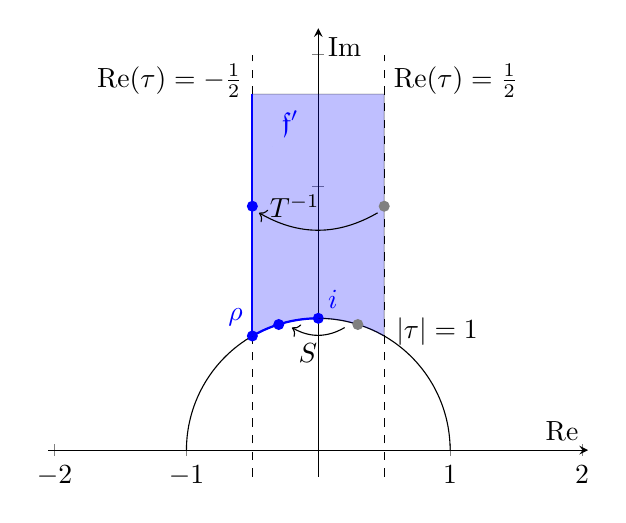
\begin{tikzpicture}
        \begin{axis}[
            axis lines=center,
            xlabel=$\text{Re}$,
            ylabel=$\text{Im}$,
            xmin=-1.5, xmax=1.5,
            ymin=-0.2, ymax=3.2, % Adjusted ymax
            axis equal,
            legend pos=outer north east,
            legend style={draw=none},
            yticklabels={$0$, $0$, , ,}
        ]
    
        % Draw x-axis and y-axis
        \draw[-] (axis cs: -1.5,0) -- (axis cs: 1.5,0) node[below right] {};
        
        % Draw y-axis with cutoff
        \ifnum\pdfstrcmp{\pgfkeysvalueof{/pgfplots/ymin}}{-0.2}>0
            \draw[-] (axis cs: 0,-0.2) -- (axis cs: 0,3) node[above left] {$y$};
        \fi
    
        % Draw semicircle
        \addplot[domain=0:180, samples=100, black] ({cos(x)}, {sin(x)});
        \node[black] at (axis cs: 0.9, 0.9) {$|\tau| = 1$};
    
        % Draw lines x=1/2 and x=-1/2 with cutoff
        \ifnum\pdfstrcmp{\pgfkeysvalueof{/pgfplots/xmin}}{-0.2}>0
            \draw[dashed] (axis cs: 0.5,-0.2) -- (axis cs: 0.5,3) node[below right] {$\text{Re}(\tau)=\frac{1}{2}$};
            \draw[dashed] (axis cs: -0.5,-0.2) -- (axis cs: -0.5,3) node[below left] {$\text{Re}(\tau)=-\frac{1}{2}$};
        \fi

        % Mark the point (0,1) and label it as i (changed coordinates)
        \fill[blue] (axis cs:0,1) circle[radius=2pt] node[above right,blue] {$i$};

        % Mark the point (-1/2, sqrt(3)/2) and label it as \rho
        \fill[blue] (axis cs:-0.5,{sqrt(3)/2}) circle[radius=2pt] node[above left,blue] {$\rho$};
    
        \coordinate (A) at (axis cs:0.5, 0.866);
        \coordinate (A2) at (axis cs:0.4, 0.916);
        \coordinate (A3) at (axis cs:0.3, 0.953);
        \coordinate (A4) at (axis cs:0.2, 0.9797);
        \coordinate (A5) at (axis cs:0.1, 0.99498);
        \coordinate (A6) at (axis cs:0, 1);
        \coordinate (A10) at (axis cs:-0.4, 0.916);
        \coordinate (A9) at (axis cs:-0.3, 0.953);
        \coordinate (A8) at (axis cs:-0.2, 0.9797);
        \coordinate (A7) at (axis cs:-0.1, 0.99498);
        \coordinate (B) at (axis cs:-0.5, 0.866);
        \coordinate (C) at (axis cs:-0.5, 2.7);
        \coordinate (D) at (axis cs:0.5, 2.7);

        % Draw the lines connecting the points
        \draw[fill=blue, opacity=0.25, name path=ABCD] (A) -- (A2) -- (A3) -- (A4) -- (A5) -- (A6) -- (A7) -- (A8) -- (A9) -- (A10) -- (B) -- (C) -- (D) -- cycle;

        \coordinate (B1) at (axis cs: -0.5, 0.866);
        \coordinate (B2) at (axis cs: -0.5, 2.7);
        \draw[blue, thick] (B1) -- (B2);

        \addplot[domain=90:120, samples=100, blue, thick] ({cos(x)}, {sin(x)});

        \coordinate (C1) at (axis cs: 0.45, 1.8);
        \coordinate (C2) at (axis cs: -0.45, 1.8);
        \fill[gray] (axis cs: 0.5, 1.85) circle[radius=2pt];
        \fill[blue] (axis cs: -0.5, 1.85) circle[radius=2pt];
        \draw[->, bend left=30] (C1) to node[pos = 0.7, above] {$T^{-1}$} (C2);

        \coordinate (D1) at (axis cs: 0.2, 0.9297);
        \coordinate (D2) at (axis cs: -0.2, 0.9297);
        \fill[gray] (axis cs: 0.3, 0.953) circle[radius=2pt];
        \fill[blue] (axis cs: -0.3, 0.953) circle[radius=2pt];
        \draw[->, bend left=30] (D1) to node[pos = 0.7, below] {$S$} (D2);

        \fill[blue] (axis cs:-0.35,2.3) circle[radius=0pt] node[above right,blue] {$\mathfrak{f}'$};

        \end{axis}
    \end{tikzpicture}    
\end{center}

\begin{prop}
    Let $G = \Gamma(1)/\{\pm I\}$. Then
    \begin{enumerate}[(i)]
        \item $\forall \tau \in \mathfrak{h}, \tau$ is $\Gamma(1)$--conjugate to an element of $\mathfrak{f}'$.
        \item If $\tau, \tau' \in \mathfrak{f}'$ are $\Gamma(1)$--conjugate, then $\tau = \tau'$.
        \item If $\tau \in \mathfrak{f'}$, then $\text{Stab}_G(\tau)$ is trivial, except in the two cases $\text{Stab}_G(i) = \langle S \rangle$ and $\text{Stab}_G(\rho) = \langle ST \rangle$, where $\rho = e^{2\pi i / 3}$.
        \item $\Gamma(1)$ is generated by $S$ and $T$.
    \end{enumerate}
\end{prop}
\begin{proof}
    Let $H$ be the subgroup of $G$ generated by $S$ and $T$.
    \begin{claim*}
        Every $\tau \in \mathfrak{h}$ is $H$--conjugate to an element of $\mathfrak{f}'$.
    \end{claim*}
    \begin{proof}
        By our above observation and since $S,T \in H$, it suffices to prove that every $\tau \in \mathfrak{h}$ is $H$--conjugate to $\mathfrak{f}$. Take $\tau \in \mathfrak{h}$. Recall that if $\gamma = \begin{pmatrix} a & b\\c &d \end{pmatrix} \in SL_2(\mathbb{Z})$, then $\text{Im}(\gamma \tau) = \frac{\text{Im}(\tau)}{|c \tau + d|^2}$. 
        \vspace{1mm}
         
        In particular, $\forall R \ge 0$, the intersection $H \tau \cap \{\text{Im}(\tau') > R\}$ is finite, since $\text{Im}(\gamma \tau) > R \iff |c \tau + d|^2 < \frac{\text{Im}(\tau)}{R}$, but $\Lambda_\tau = \mathbb{Z} \tau \oplus \mathbb{Z}$ is a lattice, so the set $\{(c,d) \in \mathbb{Z}^2 \mid |c \tau +d| < R'\}$ is finite. 
        \vspace{1mm}
         
        So there exists $h \in H$ such that $\text{Im}(h \tau) \ge \text{Im}(h' \tau) ~\forall h' \in H$. After replacing $\tau$ by $h \tau$, we can assume $\text{Im}(\tau) \ge \text{Im}(h \tau) ~\forall h \in H$. Since acting by $T$ does not change $\text{Im}(\tau)$, we can also assume $\text{Re}(\tau) \in \left[-\frac{1}{2},\frac{1}{2}\right]$. We have $\text{Im}(\tau) \ge \text{Im}(S \tau) = \frac{\text{Im}(\tau)}{|\tau|^2} \implies |\tau|\ge 1$, proving the claim and (i).
    \end{proof}
    Now take $\tau, \tau' \in \mathfrak{f}'$ and suppose $\gamma \tau = \tau'$ for some $\gamma = \begin{pmatrix} a & b \\ c & d \end{pmatrix} \in \Gamma(1)$. We want to show that either $\gamma = \pm I$ or $\tau = i, \rho$. 
    \vspace{1mm}
     
    WLOG assume $\text{Im}(\tau') = \text{Im}(\gamma \tau) \ge \text{Im}(\tau)$, i.e. $\text{Im}(\gamma \tau) = \frac{\text{Im}(\tau)}{|c \tau + d|^2} \ge \text{Im}(\tau)$, so $|c \tau +d| \le 1$. However, if $\tau \in \mathfrak{f}'$, then $\text{Im}(\tau) \ge \frac{\sqrt{3}}{2}$ with equality if and only if $\tau = \rho$. Hence $|c \tau + d| \ge |c| \text{Im}(\tau) \ge |c|\frac{\sqrt{3}}{2} \implies |c|\le \frac{2}{\sqrt{3}} \implies |c| = 0, 1 \implies c = 0$ or $c = \pm 1$. 
    \begin{itemize}
        \item If $c=0$, then $\gamma =\begin{pmatrix} a&b\\0&d \end{pmatrix}$, so $ad = 1 \implies a = d = \pm 1$, so $\gamma = \pm T^m$ for $m \in \mathbb{Z}$. However, $T$ acts on $\mathfrak{f}'$ by shifting the real part, so it can only stay in $\mathfrak{f}'$ if $m = 0$ (as $\text{Re}(\mathfrak{f}') \in \left[-\frac{1}{2},\frac{1}{2}\right)$), so $\gamma = \pm I$ and $\tau' = \tau$.
        \item If $c=1$, then $\gamma = \begin{pmatrix} a & b\\1 & d \end{pmatrix}$ and $|\tau +d|\le 1$. By drawing another picture, we see that the only circles centered at integers of radius 1 which intersect $\mathfrak{f}'$ are centered at $-d = 0, -d = -1$. Hence either $d = 0$, whence $|\tau|=1$, or $d=1$, whence $\tau = \rho$.
        \begin{itemize}
            \item If $c=1, d= 0, |\tau|=1$, then $\gamma = \begin{pmatrix} a & b \\ 1& 0 \end{pmatrix} = \begin{pmatrix} a & -1 \\ 1 & 0 \end{pmatrix}$ since the determinant must be 1. Then $\gamma \tau =  \frac{a \tau - 1}{\tau} = a -\frac{1}{\tau} = a - \overline{\tau}$, so $\text{Re}(\gamma\tau) = a - \text{Re}(\tau) \in \text{Re}(\mathfrak{f}' \cap \{|\tau|=1\}) = \left[-\frac{1}{2}, 0\right]$. However, we also have $\text{Re}(\gamma \tau) \in a - \left[-\frac{1}{2},0\right] = a + \left[0,\frac{1}{2}\right]$. \vspace{1mm}
             
            The intersection $\left[-\frac{1}{2}, 0 \right] \cap \left(a + \left[0, \frac{1}{2}\right]\right)$ can be nonempty only if either $a=0$, whence $\text{Re}(\gamma \tau) = \text{Re}(\tau) = 0$, so $\tau = \gamma \tau = i$, or $a = -1$, whence $\text{Re}(\tau) = \text{Re}(\gamma \tau) = -\frac{1}{2}$, so $\tau = \gamma \tau = \rho$. 
            \vspace{1mm}
             
            If $a=0$, then $\gamma = \begin{pmatrix} 0  & -1 \\ 1 & 0 \end{pmatrix} = -S$, which stabilizes $i$, and $\langle -S \rangle = \langle S \rangle$.
            \vspace{1mm}
             
            If $a=-1$, then $\gamma = \begin{pmatrix} -1 & -1 \\ 1 & 0 \end{pmatrix} = (ST)^2$, which stabilizes $\rho$, and $(ST)^3 = I$, so $\langle (ST)^2 \rangle = \langle ST \rangle$.
            \item If $c=1, d=1, \tau = \rho$, then $\gamma = \begin{pmatrix} a & b \\1 & 1 \end{pmatrix}$, so $\rho = \gamma \rho = \frac{a \rho + b}{\rho + 1}$. We have $\rho^2 + \rho + 1 = 0$, so $\rho^2 + \rho = -1$, so $a \rho + b = \rho^2 + \rho = -1$. But $a, b \in \mathbb{Z}$ and $1,\rho$ are linearly independent over $\mathbb{R}$, so $a = 0, b = -1$, so $\gamma = \begin{pmatrix} 0 & -1 \\ 1 & 1 \end{pmatrix} = -ST$, which stabilizes $\rho$.
        \end{itemize}
        \item If $c = -1$, we can reduce this to the case $c=1$ by replacing $\gamma$ with $-\gamma$.
    \end{itemize}
    We have now shown the first three parts of the proposition. It remains to show the last part, i.e. $\Gamma(1) = \langle S,T \rangle$. Since $S^2 = -I$, it is enough to show that $H = G$. Choose $\tau \in \text{Int}(f)$, so $\text{Stab}_G(\tau) = \{I\}$. Let $g \in G$. By our claim proving (i), $\exists h \in H$ such that $hg \tau  \in \mathfrak{f}'$. We must therefore have $hg \tau = \tau$, hence $h g  \in \text{Stab}_G(\tau) = \{I\}$, so $g = h^{-1} \in H$.
\end{proof}

\marginpar{13 Oct 2022, Lecture 4}

\textbf{Notation.} We write $e_{\tau} = |\text{Stab}_G(\tau)|$.
\vspace{1mm}
 
Let $f$ be a nonzero modular function of weight $k$, level $\Gamma(1)$. If $\tau \in \mathfrak{h}$, then $v_{\tau}(f)$ is the order of $f$ at $\tau$ (the unique $n \in \mathbb{Z}$ such that $f(z) = (z-\tau)^n g(z)$ for some meromorphic $g$ that is holomorphic and non--vanishing at $\tau$). We define $v_{\infty}(f)$ to be the order of $f$ at infinity, i.e. $v_{\infty}(f)=v_0(\tilde{f})$ for $\tilde{f}$ the meromorphic function in $D(0,1)$ with $f(\tau) = \tilde{f}(e^{2\pi i \tau})$.

\begin{prop}
    Let $f$ be a nonzero modular function of weight $k$, level $\Gamma(1)$. Then 
    \begin{align*}
        \sum_{ \tau \in \Gamma(1)\setminus \mathfrak{h}}^{} \frac{1}{e_{\tau}}v_\tau(f) + v_\infty(f) = \frac{k}{12}.
    \end{align*}
\end{prop}
\begin{proof}
    We first check that the sum is well--defined: 
    \begin{itemize}
        \item If $\tau \in \mathfrak{h}$, then $e_\tau, v_{\tau}(f)$ only depend on the $\Gamma(1)$--orbit of $\tau$. This is because if $\gamma \in \Gamma(1)$ and $\tau \in \mathfrak{h}$, then $\text{Stab}_{\Gamma(1)}(\tau)$ and $\text{Stab}_{\Gamma(1)}(\gamma \tau)$ are conjugate subgroups of $\Gamma(1)$, so $e_{\tau} = e_{\gamma \tau}$. On the other hand, $f(\gamma \tau) = f(\tau) j(\gamma, \tau)^k$ and $j(\gamma, \tau)$ is holomorphic and non--vanishing on $\mathfrak{h}$, so $v_{\gamma \tau}(f) = v_{\tau}(f)$.
        \item The sum only has a finite number of nonzero terms, since if $f$ is a modular function and $\tilde{f}$ is a meromorphic function on $D(0,1)$, then $\exists \delta > 0$ such that $\tilde{f}$ is holomorphic and non--vanishing in $D^*(0,\delta)$. Thus $\exists R > 0$ such that $f$ is holomorphic and non--vanishing in $\{\tau \in \mathfrak{h} \mid \text{Im}(\tau)>R\}$. Hence to show the sum is finite, it suffices to show that $f$ only has a finite number of zeroes and poles in $\mathfrak{f}$ (as $\mathfrak{f}$ intersects every $\Gamma(1)$--orbit), for which it suffices to show that $f$ has a finite number of zeroes and poles in $\mathfrak{f} \cap \{\tau \in \mathfrak{h} \mid  \text{Im}(\tau)\le R\}$, which is true as the set is compact (closed and bounded) and the zeroes and poles of $f$ are discrete.
    \end{itemize}
    To prove the identity, we use contour integration. Setup: if $U \subset \mathbb{C}$ is an open subset, $f : U \to \mathbb{C}$ is holomorphic and $\gamma:[0,1] \to U$ is a path, then $$\int_{\gamma}^{} f(z)\mathrm{d}z = \int_{t=0}^{1} f(\gamma(t))\gamma'(t)\mathrm{d}t.$$ We have the pullback formula: if $u : U \to V$ is a holomorphic map between open subsets of $\mathbb{C}$, $g : V \to \mathbb{C}$ is holomorphic and $\gamma$ is a path in $U$, then $$\int_{u \circ \gamma}^{} g(z)\mathrm{d}z = \int_{\gamma}^{} u^*(g(z)\mathrm{d}z) = \int_{\gamma}^{} g(u(z))u'(z)\mathrm{d}z.$$ A particularly nice case: if $g(z)=h'(z)/h(z)$, then $g(z)\mathrm{d}z = d \log h$, so $\int_{u \circ \gamma}^{}d \log h = \int_{\gamma}^{} u^*(d \log h) = \int_{\gamma}^{} d(\log h \circ u) = \int_{\gamma}^{} \frac{(h \circ u)'(z)}{(h \circ u)(z)}\mathrm{d}z$.
    \vspace{1mm}
     
    We also have (Cauchy's) argument principle: if $U \subset \mathbb{C}$ is a simply connected open subset, $\gamma \subset U$ is a simple positvely oriented closed path and $g$ is a meromorphic function in $U$ with no zeroes or poles on $\gamma$, then $$\frac{1}{2\pi i} \oint_{\gamma} d \log g = \frac{1}{2\pi i} \oint_{\gamma} \frac{g'(z)}{g(z)}\mathrm{d}z = \sum_{a \in \text{Int}(\gamma)}^{} v_a(g).$$
    We now apply this to our modular function $f$. Choose $R>0$ such that $f$ has no zeroes or poles in $\{\tau \in \mathfrak{h} \mid \text{Im}(\tau)\ge R\}$. We consider $\frac{1}{2\pi i}\oint_{\gamma} d \log f$, where $\gamma$ is the contour $ABCDE$.
    
    \begin{center}
        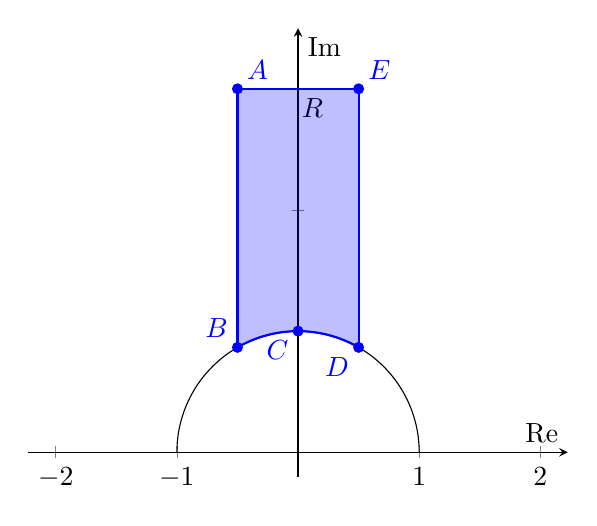
\begin{tikzpicture}
            \begin{axis}[
                axis lines=center,
                xlabel=$\text{Re}$,
                ylabel=$\text{Im}$,
                xmin=-1.5, xmax=1.5,
                ymin=-0.2, ymax=3.5, % Adjusted ymax
                axis equal,
                legend pos=outer north east,
                legend style={draw=none},
                yticklabels={$0$, $0$, , ,$R$},
                yticklabel style={below right},
            ]
        
            % Draw x-axis and y-axis
            \draw[-] (axis cs: -1.5,0) -- (axis cs: 1.5,0) node[below right] {};
            
            % Draw y-axis with cutoff
            \ifnum\pdfstrcmp{\pgfkeysvalueof{/pgfplots/ymin}}{-0.2}>0
                \draw[-] (axis cs: 0,-0.2) -- (axis cs: 0,3) node[above left] {$y$};
            \fi
        
            % Draw semicircle
            \addplot[domain=0:180, samples=100, black] ({cos(x)}, {sin(x)});
            \node[black] at (axis cs: 0.9, 0.9) {};
        
            % Draw lines x=1/2 and x=-1/2 with cutoff
            % \ifnum\pdfstrcmp{\pgfkeysvalueof{/pgfplots/xmin}}{-0.2}>0
            %     \draw[dashed] (axis cs: 0.5,-0.2) -- (axis cs: 0.5,2.8) node[below right] {$\text{Re}(\tau)=\frac{1}{2}$};
            %     \draw[dashed] (axis cs: -0.5,-0.2) -- (axis cs: -0.5,2.8) node[below left] {$\text{Re}(\tau)=-\frac{1}{2}$};
            % \fi
    
            % Mark the point (0,1) and label it as i (changed coordinates)
            \fill[blue] (axis cs:-0.5,3) circle[radius=2pt] node[above right,blue] {$A$};

            \fill[blue] (axis cs:0.5,3) circle[radius=2pt] node[above right,blue] {$E$};
            
            \fill[blue] (axis cs:0,1) circle[radius=2pt] node[below left,blue] {$C$};
    
            % Mark the point (-1/2, sqrt(3)/2) and label it as \rho
            \fill[blue] (axis cs:-0.5,{sqrt(3)/2}) circle[radius=2pt] node[above left,blue] {$B$};

            \fill[blue] (axis cs:0.5,{sqrt(3)/2}) circle[radius=2pt] node[below left,blue] {$D$};
        
            \coordinate (A) at (axis cs:0.5, 0.866);
            \coordinate (A2) at (axis cs:0.4, 0.916);
            \coordinate (A3) at (axis cs:0.3, 0.953);
            \coordinate (A4) at (axis cs:0.2, 0.9797);
            \coordinate (A5) at (axis cs:0.1, 0.99498);
            \coordinate (A6) at (axis cs:0, 1);
            \coordinate (A10) at (axis cs:-0.4, 0.916);
            \coordinate (A9) at (axis cs:-0.3, 0.953);
            \coordinate (A8) at (axis cs:-0.2, 0.9797);
            \coordinate (A7) at (axis cs:-0.1, 0.99498);
            \coordinate (B) at (axis cs:-0.5, 0.866);
            \coordinate (C) at (axis cs:-0.5, 3);
            \coordinate (D) at (axis cs:0.5, 3);
            \coordinate (E) at (axis cs:0.5, 3);
    
            % Draw the lines connecting the points
            \draw[fill=blue, opacity=0.25, name path=ABCD] (A) -- (A2) -- (A3) -- (A4) -- (A5) -- (A6) -- (A7) -- (A8) -- (A9) -- (A10) -- (B) -- (C) -- (E) -- (D) -- cycle;
    
            \coordinate (B1) at (axis cs: -0.5, 0.866);
            \coordinate (B2) at (axis cs: -0.5, 3);
            \draw[blue, thick] (B1) -- (B2) -- (E) -- (A);
                
            
            \addplot[domain=60:120, samples=100, blue, thick] ({cos(x)}, {sin(x)});    
            \end{axis}
        \end{tikzpicture}    
    \end{center}

    By choice of $R$, there are no zeroes or poles of $f$ on $AE$. We first consider the case where $f$ has no zeroes or poles at all on $\gamma$. Then the argument principle gives $$\frac{1}{2\pi i}\oint_{\gamma} d \log f = \frac{1}{2\pi i} \int_{AB}^{} +\int_{BC}^{} +\int_{CD}^{} +\int_{DE}^{} +\int_{EA}^{} d \log f = \sum_{\tau \in \Gamma(1)\setminus \mathfrak{h}}^{} \frac{1}{e_{\tau}}v_\tau(f) $$
    (as $v_\tau(f) \neq 0$, $e_{\tau} = 1$ under our assumptions).
    \vspace{1mm}
     
    Apply the pullback formula with $u(\tau) = \tau+1$. Then $u(AB) = ED$, $f \circ u = f$, so $$\int_{u(AB)}^{} d \log f = \int_{AB}^{} d \log f \circ u = \int_{AB}^{} d \log f = \int_{ED}^{} d \log f = - \int_{DE}^{} d \log f.$$
    Hence $\int_{AB}^{} + \int_{DE}^{} d \log f = 0$.
    \vspace{1mm}
     
    Now take $q = e^{2\pi i \tau}$, so $f = \tilde{f} \circ q$ and $q(AE)$ is a positively oriented circle around 0 in $D(0,1)$. So $$\frac{1}{2\pi i} \int_{q(AE)}^{} d \log \tilde{f} = v_{\infty}(f) = \frac{1}{2\pi i} \int_{AE}^{} d \log \tilde{f} \circ q = \frac{1}{2\pi i}\int_{AE}^{} d \log f.$$ 
    \vspace{1mm}
     
    Now take $v(\tau) = S(\tau) = -\frac{1}{\tau}$. Then $v(BC) = DC$ and we know $f|_k[S](\tau) = f\left(-\frac{1}{\tau}\right)\tau^{-k} = f(\tau)$, so $f \circ v = f(\tau)\tau^k$. Hence 
    \begin{align*}
        &\int_{DC}^{} d \log f = \int_{v(BC)}^{} d \log f = \int_{BC}^{} d \log (f \circ v) = \int_{BC}^{} d \log(f(\tau)\tau^k) \\ =& \int_{BC}^{} d \log f + k d \log \tau = \int_{BC}^{} d \log f + k(\log C - \log B)
    \end{align*}
    where here $\log$ is any branch of the logarithm defined on $BC$. But $B = \rho, C = i$, so $\log B = i \frac{2\pi}{3}$ and $\log C = i \frac{\pi}{2}$. Hence \[
    \int_{CD}^{} d \log f = - \int_{DC}^{} d \log f + k\left(\frac{2\pi i }{3} - \frac{2 \pi i }{4}\right),
    \]
    giving \[
    \int_{BC}^{} +\int_{CD}^{} d \log f = 2\pi i k \frac{1}{12}.
    \]
    We have 
    \begin{align*}
        \sum_{\Gamma(1)\setminus \mathfrak{h}}^{} \frac{1}{e^{\tau}} v_\tau(f) =& \frac{1}{2\pi i } \left(\int_{AB}^{} +\int_{BC}^{} +\int_{CD}^{} +\int_{DE}^{} +\int_{EA}^{} d \log f \right) \\
        =& \frac{1}{2\pi i} \left( 0 + \frac{k}{12} + 0 - v_{\infty}(f) \right) \\
        &\implies \sum_{ \tau \in \Gamma(1)\setminus \mathfrak{h}}^{} \frac{1}{e_{\tau}}v_\tau(f) + v_\infty(f) = \frac{k}{12}.
    \end{align*}
    This finishes the proof in the case where there are no zeroes or poles. If there are zeroes or poles on $\gamma$, we need to modify the contour. For example, if there's a zero or a pole at a point $P$ on $AB$, then consider the contour $\gamma'$, which is just $\gamma$ but with a small semicircle around our (discrete) pole, which satisfies the property that $f$ has no zeroes or poles on $\gamma'$. The trickiest case is when there is a zero or pole at $B = \rho$ or $C = i$. This is Q3 on example sheet 1. 
\end{proof}

\marginpar{16 Oct 2022, Lecture 5}

\begin{example}
    Take $k=4$, $f = E_4 \in M_{4}(\Gamma(1))$. Hence $\forall \tau \in \mathfrak{h}, v_{\tau}(E_4)\ge 0$ (as it is holomorphic in $\mathfrak{h}$). We know $E_4(\tau) = 1 + \sum_{n\ge 1}^{} a_nq^n$, so $E_4(\infty) \neq 0$ and $v_{\infty}(E_4) = 0$. Hence our formula gives 
    \begin{align*}
        \sum_{\tau \in \Gamma(1)\setminus \mathfrak{h}}^{} \frac{1}{e_{\tau}}v_{}(E_4) = \frac{1}{3} v_{\rho}(E_4) + \frac{1}{2}v_i(E_4) + \sum_{\tau \in \Gamma(1)\setminus \mathfrak{h}, \tau \not\sim \rho,i}^{} v_{\tau}(E_4) = \frac{1}{3}.
    \end{align*}
    So we have $\frac{a}{3}+\frac{b}{2}+c = \frac{1}{3}$, where $a,b,c \in \mathbb{Z}_{\ge 0}$, which gives the only solution $a=1, b=c=0$, so $E_4(\rho)=0$ and $E_4(\tau) \neq 0$ if $\tau \not\in \Gamma(1)\rho$.
    \vspace{1mm}
     
    If $k=6$, $f = E_6$, then we get \[
    \frac{1}{3}v_{\rho}(E_6) + \frac{1}{2}v_i(E_6) + \sum_{\tau \not\sim \rho,i}^{} v_{\tau}(E_6) = \frac{6}{12} = \frac{1}{12},
    \]
    so this forces $v_{\rho}(E_6) = 0$, $v_{i}(E_6) = 1$, $v_{\tau}(E_6) \neq 0$ if $\tau \not\sim \rho$ and $\tau \not\sim i$, so $E_6(i) = 0$, $E_6(\tau) \neq 0$ if $\tau \not\sim \rho,i$.
\end{example}
Recall $\Delta = \frac{E_4^3 - E_6^2}{1728} \in S_{12}(\Gamma(1))$. This is nonzero since $\Delta(\rho) = \frac{E_4(\rho)^3 - E_6(\rho)^2}{1728}  = -\frac{E_6(\rho)^2}{1728} \neq 0$. We also have $v_{\infty}(\Delta)\ge 1$ by construction, so plug in $\Delta$ to our formula to get 
\begin{align*}
    \sum_{\tau}^{} \frac{1}{e_{\tau}}v_{\tau}(\Delta) + v_{\infty}(\Delta) = 1,
\end{align*}
so $v_{\infty}(\Delta) = 1$, so $\Delta$ has a simple zero at $\infty$ and $\Delta$ is nonvanishing in $\mathfrak{h}$.

\begin{theorem}
    Let $k \in 2\mathbb{Z}$. Then:
    \begin{enumerate}[(1)]
        \item If $k<0$ or $k=2$, then $M_k(\Gamma(1)) = 0$; and $M_0(\Gamma(1)) = \mathbb{C} \cdot 1$.
        \item If $4\le k\le 10$, then $M_k(\Gamma(1)) = \mathbb{C} \cdot E_k$. 
        \item For any $k$, multiplication by $\Delta$ gives an isomorphism $M_k(\Gamma(1)) \stackrel{\times \Delta}{\to}  S_{k+12}(\Gamma(1))$.
    \end{enumerate}
\end{theorem}
\begin{proof}
    \begin{enumerate}[(1)]
        \item Let $f \in M_k(\Gamma(1))$ be nonzero. Then $\sum_{}^{} \frac{1}{e_{\tau}}v_{\tau}(f) + v_{\infty}(f) = \frac{k}{12}$. Note the LHS is $\ge 0$, but for $k<0$, the RHS is $<0$. If $k=2$, then we get the equation $\frac{a}{3}+\frac{b}{2}+c = \frac{1}{6}$ for $a,b,c \in \mathbb{Z}_{\ge 0}$, which has no solutions.
        \vspace{1mm}
         
        Suppose $f \in M_0(\Gamma(1)) \setminus \mathbb{C}\cdot 1$. Then $f - f(\infty) \cdot 1  \in S_0(\Gamma(1))$ is a nonzero function (here 1 is the constant function 1). Then $\sum_{\tau}^{} \frac{1}{e_{\tau}}v_{\tau}(f-f(\infty)\cdot 1) + \underbrace{v_{\infty}(f-f(\infty)\cdot 1)}_{\ge 1} = 0$, a contradiction, so $M_0(\Gamma(1)) = \mathbb{C}\cdot 1$.
        \item Let $4\le k\le 10$ and $f \in M_k(\Gamma(1))$. Consider $f - f(\infty)\cdot E_k \in S_k(\Gamma(1))$. If this is nonzero, then \[
        \sum_{\tau}^{} \frac{1}{e_\tau}v_{\tau}(f-f(\infty)\cdot E_k) + \underbrace{v_{\infty}(f-f(\infty)\cdot E_k)}_{\ge 1} = \frac{k}{12}<1,
        \]
        a contradiction. So $f = f(\infty)\cdot E_k$.
        \item Our map $\times \Delta : M_k(\Gamma(1)) \to S_{k+12}(\Gamma(1))$ is a well--defined $\mathbb{C}$--linear map. It is injective, since if $\Delta f = 0$, then $f = 0$ (as $\Delta$ is nonvanishing in $\mathfrak{h}$). For surjectivity, if $f \in S_{k+12}(\Gamma(1))$, then $\frac{f}{\Delta}$ is holomorphic in $\mathfrak{h}$ and invariant under the weight $k$ action of $\Gamma(1)$. 
        \vspace{1mm}
         
        We need to show $\frac{f}{\Delta}$ is holomorphic at $\infty$, as then $\frac{f}{\Delta} \in M_k(\Gamma(1))$, so $f = \frac{f}{\Delta}f \in \text{Im}(\times \Delta)$. Hence we need $v_{\infty}\left(\frac{f}{\Delta}\right) \ge 0$. But $v_{\infty}\left(\frac{f}{\Delta}\right) = \underbrace{v_{\infty}(f)}_{\ge 1} - \underbrace{v_{\infty}(\Delta)}_{=1} \ge 0$, so we're done.
    \end{enumerate}
\end{proof}
\begin{cor}
    If $k \in 2\mathbb{Z}$, $k\ge 0$, then $M_k(\Gamma(1))$ is finite--dimensional and $$\text{dim}_{\mathbb{C}}M_k(\Gamma(1)) = \begin{cases}
        \left\lfloor \frac{k}{12} \right\rfloor + 1 & k \not\equiv 2 \pmod{12}.\\
        \left\lfloor \frac{k}{12} \right\rfloor & k \equiv 2 \pmod{12}.
    \end{cases}$$
\end{cor}
\begin{proof}
    We proved this for $0\le k \le 10$. In general, use induction on $k$: we need to show that for $k\ge 0$, $\text{dim}_{\mathbb{C}}M_{k+12}(\Gamma(1)) = \text{dim}_{\mathbb{C}}M_k(\Gamma(1)) + 1$.
    \vspace{1mm}
     
    We know $E_{k+12} \in M_{k+12}(\Gamma(1))$, so $M_{k+12}(\Gamma(1)) = \mathbb{C} E_{k+12} \oplus S_{k+12}(\Gamma(1))$. But this equals $\mathbb{C} E_{k+12} \oplus \Delta M_k(\Gamma(1))$, so $\text{dim}_{\mathbb{C}} M_{k+12}(\Gamma(1)) = 1 + \text{dim}_{\mathbb{C}}M_k(\Gamma(1))$.
\end{proof}
\begin{example}
    We have $E_4^2 \in M_8(\Gamma(1)) = \mathbb{C} E_8$. So there is a relation between $E_4^2$ and $E_8$ (in this case, one is a scalar multiple of the other), but we have $E_8(\infty) = 1 = E_4(\infty)^2 \implies E_4^2 = E_8$.
    \vspace{1mm}
     
    Similarly, $E_4E_6 \in M_{10}(\Gamma(1)) = \mathbb{C} E_{10}$, so we find  $E_4 E_6 = E_{10}$.
\end{example}
\begin{cor}
    If $k \in 2\mathbb{N}$, then $M_k(\Gamma(1))$ is spanned as a $\mathbb{C}$--vector space by $\{E_4^aE_6^b \mid a,b \in \mathbb{Z}_{\ge 0}, 4a+6b=k\}$. In other words, if $\mathcal{M} = \oplus_{k \in \mathbb{Z}}M_k(\Gamma(1))$, then $\mathcal{M}$ is a graded $\mathbb{C}$--algebra generated by $E_4$ and $E_6$.
\end{cor}
\begin{proof}
    We proved this for $0\le k\le 10$. If $k\ge 12$, then $$M_k(\Gamma(1)) = \mathbb{C} E_k \oplus \Delta M_{k-12}(\Gamma(1)) = \mathbb{C} f \oplus \Delta M_{k-12}(\Gamma(1))$$ for any $f \in M_k(\Gamma(1))$ such that $f(\infty) \neq 0$ by the same argument. We can always find some $A,B \in \mathbb{Z}_{\ge 0}$ such that $4A+6B = k$, so $E_4^A E_6^B \in M_k(\Gamma(1))$ and $(E_4^A E_6^B)(\infty) \neq 0$. Now by induction, $M_{k-12}(\Gamma(1)) = \langle E_4^a E_6^b \mid 4a+6b = k-12 \rangle$, so $\Delta M_{k-12}(\Gamma(1)) = \langle \Delta E_4^a E_6^b \mid 4a+6b = k -12 \rangle$. But $\Delta \in \langle E_4^3, E_6^2 \rangle$, so \[
    \Delta M_{k-12}(\Gamma(1)) = \langle E_4^a E_6^b \mid 4a+6b = k \rangle
    \]
    and $E_4^A E_6^B \in \langle E_4^a E_6^b \mid 4a+6b = k \rangle$, so $M_k(\Gamma(1)) = \langle E_4^a E_6^b \mid 4a+6b = k \rangle$.
\end{proof}
\begin{theorem}
    Let $j(\tau) = \frac{E_4(\tau)^3}{\Delta}$. Then $j$ is a modular function of weight $0$, level $\Gamma(1)$ which is holomorphic on $\mathfrak{h}$ and has a simple pole at $\infty$. It defines a bijection $\Gamma(1)\setminus \mathfrak{h} \to \mathbb{C}$ given by $\tau \to j (\tau)$. Moreover, every modular function of weight 0, level $\Gamma(1)$ is a rational function of $j$.\footnote{Remember that $\Gamma(1)\setminus \mathfrak{h}$ is the set of orbits of $\Gamma(1)$ under $\mathfrak{h}$.}
\end{theorem}
The interpretation of this is that it is possible to define a Riemann surface structure on $\Gamma(1)\setminus \mathfrak{h} \sqcup \{\infty\}$ such that we get a compact Riemann surface whose meromorphic functions are exactly the modular functions of weight 0. So the theorem says that this Riemann surface, called $X(1)$, is isomorphic to the Riemann sphere, and our formula says that if $\mathcal{L}$ is an invertible sheaf on a compact Riemann surface and $S$ is a meromorphic section, then $\sum_{a}^{} v_a(S) = \text{deg}(\mathcal{L})$. This is useful if we are also taking algebraic geometry.

\marginpar{18 Oct 2022, Lecture 6}

\begin{proof}
    We showed that $\Delta$ is nonvanishing in $\mathfrak{h}$ and has a simple zero at $\infty$. Hence $j$ is holomorphic in $\mathfrak{h}$ and $v_{\infty}(j)=3v_{\infty}(E_4)-v_{\infty}(\Delta) = -1$. Note that if $\gamma \in \Gamma(1)$, then $j|_0[\gamma](\tau) = j(\gamma \tau) = j(\tau)$ since the map is constant on $\Gamma(1)$--orbits. To show the map is a bijection, we need to show that $\forall z \in \mathbb{C}$, there exists a unique orbit $\Gamma(1)\cdot \tau$ such that $j(\tau)=z$, i.e. $v_\tau(j-z)>0$. \vspace{1mm}
     
    We know \[
    \sum_{\tau \in \Gamma(1)\setminus \mathfrak{h}}^{} \frac{1}{e_{\tau}} \underbrace{v_{\tau}(j-z)}_{\ge 0, \text{ as }j-z \text{ is holomorphic in }\mathfrak{h}.} = 1,
    \]
    (since $v_{\infty}(j-z) = -1$ and $\frac{k}{12}= 0$) again giving $\frac{a}{3} +\frac{b}{2}+c= 1$ for $a,b,c \in \mathbb{Z}_{\ge 0}$, $ a = v_{\rho}(j-z), b = v_{i}(j-z), c = \sum_{\tau \not\sim \rho,i}^{} v_\tau(j-z)$. This gives the solutions 
    \begin{itemize}
        \item $(a,b,c) = (0,0,1)$, so $j-z$ vanishes at a unique $\Gamma(1)\cdot \tau$.
        \item $(a,b,c) = (0,2,0)$, so $j-z$ vanishes at $i$.
        \item $(a,b,c) = (3,0,0)$, so $j-z$ vanishes at $\rho$.
    \end{itemize}
    Hence our map is bijective. Consider a nonzero modular function $f$ of weight 0. To get rid of all the poles, we can consider a product $f \cdot \prod_{i=0}^{n} \left(j(\tau)-j(a_i)\right)^{b_i}$ for $a_i \in \mathfrak{h}$, $b_i \in \mathbb{Z}_{\ge 0}$, where the $a_i$ are among the poles of $f$ in $\mathfrak{h}$. Hence to show $f$ is a rational function of $j$, it is enough to consider the case where $f$ is holomorphic in $\mathfrak{h}$. Then there exists $m\ge 0$ such that $\Delta^m f$ is holomorphic at $\infty$, so $\Delta^m f$ is holomorphic in $\mathfrak{h}$ and at $\infty$, so $\Delta^m f \in M_{12m}(\Gamma(1))$. We showed that $M_{12m}(\Gamma(1)) = \langle E_4^a E_6^b \mid 4a+6b=12m \rangle$, so $f$ is a linear combination of functions of the form $\frac{E_4^aE_6^b}{\Delta^m}$, where $4a+6b=12m$. 
    \vspace{1mm}
     
    Hence it is enough to show that $\frac{E_4^aE_6^b}{\Delta^m}$ is a rational function of $j$ where $4a+6b=12m$, $a,b \in \mathbb{Z}_{\ge 0}$. But then $2a+3b=6m$, which gives $p,q \in \mathbb{\mathbb{Z}}_{\ge 0}$ such that $a =3p, b = 2q$, so $p+q=m$. Then $$\frac{E_4^aE_6^b}{\Delta^m} = \left(\frac{E_4^3}{\Delta}\right)^p \left(\frac{E_6^2}{\Delta}\right)^q = j^p \left(\frac{E_6^2}{\Delta}\right)^q.$$ 
    As $E_4^3 - E_6^2 = 1728\Delta$, we get $j = \frac{E_6^2}{\Delta} + 1728$. So this is a rational function of $j$.
\end{proof}
\begin{prop}
    Let $k\ge 4$ be an even integer. Then $$G_k(\tau) = 2\zeta(k) + 2\frac{(2\pi i)^k}{(k-1)!} \sum_{n\ge 1}^{} \sigma_{k-1}(n)q^n$$
    where $q = e^{2\pi i \tau}$ and $\sigma_{k-1}(n) = \sum_{d \mid n}^{} d^{k-1}$.
\end{prop}
\begin{proof}
    We start from the identity $$\pi \cot (\pi \tau) = \frac{1}{\tau} + \sum_{n\ge 1}^{} \left(\frac{1}{\tau+n} + \frac{1}{\tau-n}\right).$$
    This is true for $\tau \in \mathfrak{h}$ and it is even locally uniformly convergent in $\mathfrak{h}$. We can write \[
    \pi \cot(\pi \tau) = i\pi \frac{e^{\pi i \tau} + e^{-\pi i \tau}}{e^{\pi i \tau}-e^{- \pi i \tau}} = \pi i \frac{q+1}{q-1} = -\pi i (1+q)(1-q)^{-1} = -\pi i \left(1+2\sum_{n\ge 1}^{} q^n\right).
    \]
    Differentiate term--by--term $k-1$ times. The RHS of the bottom expression is \[
    -2\pi i \left(\frac{\mathrm{d}}{\mathrm{d}\tau}\right)^{k-1}\left(\sum_{n\ge 1}^{} q^n \right) = -\left(2\pi i\right)^k \sum_{n\ge 1}^{} n^{k-1}q^n,
    \]
    while the RHS of the top expression is \[
    (-1)^{k-1}(k-1)! \left(\tau^{-k} + \sum_{n\ge 1}^{} (\tau+n)^{-k} + (\tau-n)^{-k} \right) = (-1)^{k-1}(k-1)! \sum_{n \in \mathbb{Z}}^{} (\tau+n)^{-k}.   
    \]
    Rearranging and using the fact that $k$ is even (to make the sign go away) gives \[
    \sum_{n \in \mathbb{Z}}^{} (\tau+n)^{-k} = \frac{(2\pi i)^k}{(k-1)!} \sum_{n\ge 1}^{} n^{k-1}q^n, \tau \in \mathfrak{h}.
    \]
    Then \[
    G_k(\tau) = \sum_{(m,n) \in \mathbb{Z}^2\setminus 0}^{} (m \tau + n)^{-k} = 2 \zeta(k) + \sum_{\substack{(m,n) \in \mathbb{Z}^2\setminus 0, \\m \neq 0}}^{} (m \tau + n)^{-k} = 2 \zeta(k) + 2 \sum_{m\ge 1}^{} \sum_{n \in \mathbb{Z}}^{} (m \tau + n)^{-k}.
    \]
    Plug in our identity to get 
    \begin{align*}
        G_k(\tau) =& 2 \zeta(k) + \sum_{m\ge 1}^{} \frac{(2\pi i )^k}{(k-1)!} \sum_{n\ge 1}^{} n^{k-1}q^{mn} = 2\zeta(k) + \frac{2 (2\pi i)^k}{(k-1)!} \sum_{N\ge 1}^{} \underbrace{\left(\sum_{n \mid N}^{} n^{k-1}\right)}_{=\sigma_{k-1}(N)}q^N.
    \end{align*}
\end{proof}
\begin{cor}
    $E_k(\tau) = \frac{G_k(\tau)}{2\zeta(k)} = 1 + \sum_{n\ge 1}^{} a_nq^n$ has all $a_n \in \mathbb{Q}$. Moreover, if $k=4$ or $k=6$, then $a_n \in \mathbb{Z}$.
\end{cor}
\begin{proof}
    We have $$E_k(\tau) = 1 + \frac{(2\pi i)^k}{\zeta(k)(k-1)!}\sum_{n\ge 1}^{} \sigma_{k-1}(n)q^n.$$
    Hence we need to show that $\frac{\zeta(k)}{\pi^k}$ is rational. This is on example sheet 1 (when $k$ is even). One can show that $\zeta(4) = \frac{\pi^4}{90}$ and $\zeta(6) = \frac{\pi^6}{945}$, so 
    \begin{align*}
        &E_4(\tau) = 1 + \frac{2^4 \pi^4 \cdot 90}{\pi^4 \cdot 6}\sum_{n\ge 1}^{} \sigma_3(n)q^n = 1 + 240\sum_{n\ge 1}^{} \sigma_3(n)q^n\\
        &E_6(\tau) = 1 -\frac{2^6 \pi^6 \cdot 3^3 \cdot 5 \cdot 7}{\pi^6 \cdot 5!}\sum_{n\ge 1}^{} \sigma_5(n)q^n = 1 - 504 \sum_{n\ge 1}^{} \sigma_5(n)q^n.
    \end{align*}
\end{proof}
\begin{cor}
    If $\Delta(\tau) = \sum_{n\ge 1}^{} \tau(n)q^n$ is the $q$--expansion of $\Delta$, then $\tau(1)=1$ and $\tau(n) \in \mathbb{Z} ~\forall n\ge 1$.
\end{cor}
\begin{proof}
    Write $E_4 = 1 + 240U$ and $E_6 = 1 -504V$ for $U,V = q + \ldots \in \mathbb{Z}[[q]]$. Then 
    \begin{align*}
        \Delta &= \frac{E_4^3-E_6^2}{1728} = \frac{(1+240U)^3-(1-504V)^2}{1728} \\
        &= \frac{3\cdot 240U + 3\cdot 240^2 U^2 + 240^3 U^3 + 2\cdot 504V - 504^2V^2}{1728}\\
        &= \frac{(3\cdot 240 U + 2\cdot 504 V)}{1728} + R,
    \end{align*}
    where we claim $R \in q^2\mathbb{Z}[[q]]$, but for this we just need to check that $1728 \mid 3\cdot 240^2, 1728 \mid240^3, 1728 \mid504^2$, which is true.
    \vspace{1mm}
     
    We need to check that $$\frac{(3\cdot 240 U + 2\cdot 504 V)}{1728} = \frac{2^4 \cdot 3^2\cdot 5\cdot U + 2^4 \cdot 3^2\cdot 7\cdot V}{2^6\cdot 3^3} \in \mathbb{Z}[[q]].$$ But this equals \[
    \frac{5U+7V}{12} = \frac{5(U-V)}{12} + V.
    \]
    Hence we need to check that \[
    \frac{5}{12}(\sigma_3(n)-\sigma_5(n)) \in \mathbb{Z} ~\forall n\ge 1,
    \]
    i.e. we need to check that \[
    \sigma_3(n) \equiv \sigma_5(n) \pmod{12} ~\forall n\ge 1.
    \]
    But this is true as $d^3 \equiv d^5 \pmod{12} ~\forall d \in \mathbb{N}$.
    \vspace{1mm}
     
    Finally, we compute $\tau(1) =\frac{3\cdot 240 + 2\cdot 504}{1728} = 1$. 
\end{proof}

\marginpar{20 Oct 2022, Lecture 7}

\begin{theorem}
    Let $k\ge 4$ be even and $N = \text{dim}_{\mathbb{C}}~S_k(\Gamma(1))$. Then there exists a unique basis $f_0,\ldots,f_N$ for $M_k(\Gamma(1))$ as a $\mathbb{C}$--vector space such that
    \begin{enumerate}[(a)]
        \item $\forall 0\le i\le N$, $f_i = \sum_{n\ge 0}^{} a_n(f_i)q^n$ for $a_n(f_i) \in \mathbb{Z} ~\forall n\ge 0$.
        \item If $0\le i,n\le N$, then $a_n(f_i)=\delta_{in}$.
    \end{enumerate}
\end{theorem}
So in other words, $f_i = q^i + O(q^{N+1})$. This is important because $M_k(\Gamma(1))$ has a $\mathbb{Z}$--structure, i.e. we can realize it as a tensor product $M_k(\Gamma(1)) = M_k(\Gamma(1),\mathbb{Z})\oplus \mathbb{C}$, where $M_k(\Gamma(1),\mathbb{Z}) = \{f \in M_k(\Gamma(1)) \mid \forall n\ge 0, a_n(f) \in \mathbb{Z}\}$.

\begin{proof}
    We first construct $f_0,\ldots,f_N \in M_k(\Gamma(1))$ with properties (a) and (b). Write $k = 12a + d$, for $a, d \in \mathbb{Z}_{\ge 0}$ such that $d = 14$ if $k \equiv 2 \pmod{12}$, or $0\le d\le 10$ if $d \not\equiv 2 \pmod{12}$.
    \vspace{1mm}
     
    Then $$\left\lfloor \frac{k}{12} \right\rfloor = \begin{cases}
        a & k\not\equiv 2 \pmod{12}\\
        a+1 & k \equiv 2 \pmod{12}
    \end{cases} \implies \left\lfloor a\right\rfloor = \begin{cases}
        \left\lfloor \frac{k}{12} \right\rfloor & k\not\equiv 2 \pmod{12}\\
        \left\lfloor \frac{k}{12} \right\rfloor-1 & k \equiv 2 \pmod{12}.
    \end{cases}$$
    We have $\text{dim}_{\mathbb{C}}~M_k(\Gamma(1)) = N+1 = \begin{cases}
        \left\lfloor \frac{k}{12} \right\rfloor+1 & k \not\equiv 2 \pmod{12}\\
        \left\lfloor \frac{k}{12} \right\rfloor & k \equiv 2 \pmod{12},
    \end{cases}$ 
    so $a = N$, $k = 12N + d$.
    \vspace{1mm}
     
    Now consider $A, B \in \mathbb{Z}_{\ge 0}$ such that $d = 4A + 6B$. Consider the modular forms $$g_i = \Delta^i E_4^A E_6^B E_6^{2(N-i)}$$ for $0\le i\le N$. Each $g_i$ has weight $12i + 4A + 6B + 12(N-i) = 12N + d = k$, so $g_i \in M_k(\Gamma(1))$. As $E_4, E_6, \Delta$ have $q$--expansions in $\mathbb{Z}[[q]]$, so does $g_i$. The leading term of $g_i$ is $q^i$, so the $q$--expansions look like 
    \begin{align*}
        g_0 &= 1 + a_1(g_0)q + \ldots + a_N(g_0)q^N + O(q^{N+1})\\
        &\vdots\\
        g_{N-1} &= 0 + \ldots + q_{N-1} + a_N(g_{N-1})q^N + O(q^{N+1})\\
        g_N &= 0 + \ldots + 0 + q^N + O(q^{N+1})
    \end{align*}
    We can now carry out row reduction on the $g_i$ to obtain $f_0,\ldots,f_N$ satisfying (a) and (b). For uniqueness, consider the linear functionals 
    \begin{align*}
        &a_0,\ldots,a_N : M_k(\Gamma(1)) \to \mathbb{C}\\
        &f \mapsto a_i(f), ~f = \sum_{n\ge 0}^{} a_n(f)q^n.
    \end{align*}
    Then $a_i(f_j) = \delta_{ij}$, which forces $a_0,\ldots,a_n$ to be linearly independent. Hence they form a basis of the dual vector space $M_k(\Gamma(1))^{*}$. So $f_0,\ldots,f_N$ is the dual basis of $M_k(\Gamma(1))$, and they form the unique basis with this property.
\end{proof}

\section{Hecke operators}

Hecke operators are just symmetries (linear endomorphisms) of spaces of modular forms. They can arise from either representation theory: $\Gamma(1) \le GL_2(\mathbb{Q})^{+}$, which acts on $\{f : \mathfrak{h} \to \mathbb{C}\}$ by $f \mapsto f|_k[g]$. But $M_k(\Gamma(1)) \le \{f : \mathfrak{h} \to \mathbb{C}\}^{\Gamma(1)}$, and a general group theory fact says that under suitable conditions, there's an action by a big class of operators; or from geometry: we can think of modular forms as functions on the set of lattices $\mathcal{L}$ in $\mathbb{C}$. In this course, we will follow the second point of view.
\vspace{1mm}
 
\textbf{Recall.} If $V$ is a finite--dimensional $\mathbb{R}$--vector space, then a lattice $\Lambda$ in $V$ is a subgroup $\Lambda \subset V$ which is discrete and cocompact (i.e. $V/\Lambda$ is compact).

\begin{lemma}
    A subgroup $\Lambda \le V$ is a lattice if and only if there exists a basis $e_1,\ldots,e_n$ for $V$ as a $\mathbb{R}$--vector space such that $\Lambda = \mathbb{Z} e_1 \oplus \ldots\oplus \mathbb{Z}e_n$.
\end{lemma}
\begin{proof}
    This is a question on example sheet 2.
\end{proof}
We study $\mathcal{L} = \{\Lambda \le \mathbb{C} \text{ a lattice}\}$ with its action by $\mathbb{C}^\times$, i.e. $z \Lambda = \{z \lambda \mid \lambda \in \Lambda\}$ for $z \in \mathbb{C}^\times, \Lambda \in \mathcal{L}$.

\begin{prop}
    The map $\tau \mapsto \Lambda \tau = \mathbb{Z} \tau \oplus \mathbb{Z}$ induces a bijection between $$\Gamma(1)\setminus \mathfrak{h} \leftrightarrow \mathbb{C}^\times\setminus \mathcal{L}$$ (orbits of $\Gamma(1)$ in $\mathfrak{h}$ and the set of lattices in $\mathbb{C}$ modulo scalar multiplication).
\end{prop}
\begin{proof}
    This map is well--defined, since if $\gamma = \begin{pmatrix} a & b\\ c&d \end{pmatrix} \in \Gamma(1)$, $\tau \in \mathfrak{h}$, then \[
    \Lambda_{\gamma \tau} = \mathbb{Z} \left(\frac{a \tau +b}{c \tau +d }\right) \oplus \mathbb{Z} = (c \tau + d)^{-1} \left(\mathbb{Z}(a \tau +b) \oplus \mathbb{Z}(c \tau + d)\right) = (c \tau + d)^{-1} \Lambda_{\tau}.
    \]
    For surjectivity, if $\Lambda$ is a lattice, then $\Lambda = \mathbb{Z}e_1 \oplus \mathbb{Z}e_2$ with $\text{Im}\left(\frac{e_1}{e_2}\right) \neq 0$. Swapping $e_1,e_2$ if necessary, we may assume that $\text{Im}\left(\frac{e_1}{e_2}\right)>0$. Then $\Lambda = e_2(\mathbb{Z}e_1/e_2 \oplus \mathbb{Z}) = e_1 \Lambda_\tau$ for $\tau = \frac{e_1}{e_2}$.
    \vspace{1mm}
     
    For injectivity, if $\tau,\tau'$ have the same image, then $\exists z \in \mathbb{C}^\times$ such that $\mathbb{Z}\Lambda_\tau = \Lambda_{\tau'}$, i.e. $\exists  \gamma = \begin{pmatrix} a&b\\c&d \end{pmatrix} \in GL_2(\mathbb{Z})$ such that $\tau' = az\tau + bz, 1 = cz \tau + dz$. Then $\tau' =\frac{az \tau + bz}{c z \tau + dz} = \frac{a \tau + b}{c \tau + d}$. But $\text{Im}(\tau') = \text{Im}(\gamma \tau) = \det(\gamma)\frac{\text{Im}(\tau)}{|c \tau + d|^2}$ and $\text{Im}(\tau)>0, \text{Im}(\tau')>0$, hence $\det(\gamma)>0$, so $\det(\gamma)=1$ and so $\gamma \in \Gamma(1)$. 
\end{proof}
\begin{defn}
If $k \in \mathbb{Z}$, say a function $F: \mathcal{L} \to \mathbb{C}$ is \textbf{of weight} $k$ if $\forall  z \in \mathbb{C}^\times, \Lambda \in \mathcal{L}$, $F(z \Lambda) = z^{-k}F(\Lambda)$.
\end{defn}
\begin{prop}
    Let 
    \begin{align*}
        &V_k = \{F : \mathcal{L} \to \mathbb{C} \text{ of weight }k\}.\\
        &W_k = \{f : \mathfrak{h} \to \mathbb{C} \mid \forall \gamma \in \Gamma(1), f|_k[\gamma] = f\}.
    \end{align*}
    Then the map $F \mapsto (f : \tau \mapsto F(\Lambda \tau))$ induces a $\mathbb{C}$-vector space isomorphism $V_k \to W_k$.
\end{prop}
\begin{proof}
    We first check that if $F \in V_k$, $f(\tau) = F(\Lambda \tau)$, then $f \in W_k$. If $\gamma \in \Gamma(1)$, $$f|_k[g](\tau) = f(\gamma \tau)j(\gamma,\tau)^{-k} = F(\lambda \gamma \tau)j(\gamma,\tau)^{-k} = F(j(\gamma,\tau)\Lambda_{\gamma \tau}) = F(\Lambda \tau) = f(\tau),$$
    so $j(\gamma,\tau)\Lambda_{\gamma \tau}= \Lambda_\tau$.
    \vspace{1mm}
     
    To show that the map is an isomorphism, we write down its inverse: define $\alpha:W_k \to V_k$ by $\alpha(f)(\Lambda) = e_2^{-k}f(e_1/e_2)$ if $\Lambda= \mathbb{Z}e_1 \oplus \mathbb{Z}e_2$ with $\text{Im}(e_1/e_2)>0$. This is well--defined, since if $e_1',e_2'$ is another basis with $\text{Im}(e_1'/e_2')>0$, then $\exists \gamma  = \begin{pmatrix} a&b \\c&d \end{pmatrix}\in \Gamma(1)$ such that $e_1' = ae_1 + be_2, e_2' = ce_1 + de_2$. Then 
    \begin{align*}
        e_2'^{-k} f(e_1'/e_2') &= (ce_1 + de_2)^{-k}f\left(\frac{ae_1 +be_2}{ce_1+de_2}\right) \\&= e_2^{-k}(ce_1/e_2 + d)^{-k} f \left(\frac{ae_1/e_2 + b}{ce_1/e_2+d}\right) = e_2^{-k}f\left(\frac{e_1}{e_2}\right).
    \end{align*}
    Exercise: check that the two maps are inverse to each other.
\end{proof}

\marginpar{23 Oct 2022, Lecture 8}

\begin{defn}
    Let $n \in \mathbb{N}$. The $n^{\text{th}}$ Hecke operator $T_n: V_k \to V_k$ is defined by the formula \[
    (T_n F)(\Lambda) = n^{k-1}\sum_{\Lambda' \substack{\le \\ n} \Lambda}^{} F(\Lambda').
    \]
    Here $\sum_{\Lambda' \substack{\le \\ n} \Lambda}^{}$ means summing over all subgroups $\Lambda'$ of $\Lambda$ of index $n$.
    \vspace{1mm}
     
    We also write $T_n : W_k \to W_k$ for the endomorphism arising from the isomorphism $V_k \stackrel{\sim}{\to}  W_k$.
\end{defn}
Why is $T_n$ a well--defined endomorphism of $V_k$? First of all, the sum is finite since there's a bijection 
\begin{align*}
    \{\Lambda' \le \Lambda\} &\leftrightarrow \{H \le \Lambda/n \Lambda \text{ of index }n\}\\
    \Lambda' &\mapsto \Lambda'/n \Lambda\\
    H + n \Lambda &\mapsfrom H
\end{align*}
This is well--defined, since Lagrange's theorem implies that $$\Lambda' \substack{\le \\n} \Lambda \implies n(\Lambda/\Lambda') = 0 \implies n \Lambda \le \Lambda'.$$ But $\Lambda/n \Lambda \cong \mathbb{Z}/n\mathbb{Z} \times \mathbb{Z}/n\mathbb{Z}$ is finite, so it has finitely many subgroups of index $n$.
\vspace{1mm}
 
If $\Lambda' \substack{\le  \\ n} \Lambda$, then $n \Lambda \le  \Lambda' \le \Lambda$, so $\Lambda'$ is also discrete and cocompact in $\mathbb{C}$.
\vspace{1mm}
 
We next check that $T_nF$ is of weight $k$, i.e. that $(T_nF)(z \Lambda) = z^{-k}(T_nF)(\Lambda)$. We have an isomorphism $\{\Lambda' \substack{\le \\ n} z\Lambda\} \leftrightarrow \{\Lambda' \substack{\le \\n} \Lambda\}$ given by $\Lambda' \mapsto z^{-1} \Lambda'$, so
\begin{align*}
    (T_nF)(z \Lambda) = n^{k-1}\sum_{\Lambda' \substack{\le \\ n} z\Lambda}^{} F(\Lambda') = n^{k-1} \sum_{\Lambda' \substack{\le  \\ n} \Lambda}^{} F(z \Lambda') = n^{k-1}\sum_{\Lambda' \substack{\le  \\ n} \Lambda} z^{-k}F(\Lambda') = z^{-k}(T_nF)(\Lambda).
\end{align*}
\begin{prop}
    \begin{enumerate}[(1)]
        \item If $m,n \in \mathbb{N}$ with $(m,n) = 1$, then $T_mT_n = T_{mn}$.
        \item If $p$ is a prime number and $n \in \mathbb{N}$, then $T_{p^n}T_p = T_{p^{n+1}}+p^{k-1}T_{p^{k-1}}$ (acting on $V_k$). 
    \end{enumerate}
\end{prop}
\begin{proof}
    Let $m,n \in \mathbb{N}$, not necessarily coprime. Then 
    \begin{align*}
        (T_m(T_nF))(\Lambda) &= m^{k-1}\sum_{\Lambda' \substack{\le  \\ m} \Lambda}(T_nF)(\Lambda') = (mn)^{k-1}\sum_{\Lambda' \substack{\le  \\ m} \Lambda}\sum_{\Lambda'' \substack{\le  \\ n} \Lambda'} F(\Lambda'') \\
        &=(mn)^{k-1} \sum_{\Lambda'' \substack{\le  \\ mn} \Lambda}a(\Lambda,\Lambda'')F(\Lambda''),
    \end{align*}
    where $a(\Lambda, \Lambda'') = |\{\Lambda \substack{\ge \\ m} \Lambda' \substack{\ge \\ n} \Lambda''\}| = |H \le \Lambda/\Lambda'' \mid |H| = n|$ is the number of ways to express $\Lambda'$ as an intermediate subgroup. If $(m,n) = 1$, then $a(\Lambda,\Lambda'') = 1$ for all $\Lambda'' \le \Lambda$ as any finite abelian group of order $mn$ has a unique subgroup of order $n$.
    \begin{enumerate}[(1)]
        \item In this case, we find 
        \begin{align*}
            T_m T_nF(\Lambda) = (mn)^{k-1} \sum_{\Lambda'' \substack{\le  \\ mn} \Lambda} F(\Lambda'') = (T_{mn}F)(\Lambda) \implies T_mT_n = T_{mn}.
        \end{align*}
        \item The same computation gives (for $p$ prime, $n \in \mathbb{N}$)
        \begin{align*}
            (T_{p^n}(T_p F))(\Lambda) = p^{(n+1)(k-1)} \sum_{\Lambda'' \substack{\le  \\ p^{n+1}} \Lambda} a(\Lambda,\Lambda'')F(\Lambda''),
        \end{align*}
        where $a(\Lambda,\Lambda') = |\{H \subset \Lambda/\Lambda'' \mid |H| = p\}|$. But if $\Lambda'' \substack{\le \\ p^{n+1}} \Lambda$, then $\Lambda/\Lambda''$ need not have a unique subgroup of order $p$, as $\Lambda \cong \mathbb{Z}^2$, so $\Lambda/\Lambda''$ is a finite abelian group of order $p^{n+1}$ that can be generated by 2 elements. But any such group is isomorphic to $\mathbb{Z}/p^a\mathbb{Z} \oplus \mathbb{Z}/p^b \mathbb{Z}$, where $a\ge b\ge 0$ are integers such that $a + b = n + 1$. We now split into two cases:
        \begin{itemize}
            \item $b = 0$, so $a = n+1$ and $\Lambda/\Lambda'' \cong \mathbb{Z}/p^{n+1}\mathbb{Z}$. This group is cyclic and has a unique subgroup of order $p$, so $a(\Lambda,\Lambda'') = 1$.
            \item $b>0$, so $\Lambda/\Lambda'' \cong \mathbb{Z}/p^a \mathbb{Z} \oplus \mathbb{Z}/p^b \mathbb{Z}$. Let $\Lambda/\Lambda''[p] = \{x \in \Lambda/\Lambda'' \mid px = 0\}$. This is a subgroup of $\Lambda/\Lambda''$, and \[
            \{H \le \Lambda/\Lambda'' \mid |H| = p\}  = \{H \le \Lambda/\Lambda''[p] \mid  |H| = p\}.
            \]
            Hence $\Lambda/\Lambda''[p] \cong \mathbb{Z}/p\mathbb{Z} \oplus \mathbb{Z}/p\mathbb{Z}$ from our above isomorphism. So in this case, $a(\Lambda,\Lambda'')  = |\{H \le \mathbb{Z}/p\mathbb{Z} \oplus \mathbb{Z}/p\mathbb{Z} \mid |H|= p\}|$. In other words, \[
            a(\Lambda,\Lambda') = |\mathbb{P}^1(\mathbb{F}_p)| = |\mathbb{A}^1(\mathbb{F}_p) \cup \{\infty\}| = p+1.
            \]
        \end{itemize} 
        How do we distinguish between these two cases? We will show on example sheet 2 that if $\Lambda'' \substack{\le \\ p^{n+1}}\Lambda$, then there exists a $\mathbb{Z}$--basis $e_1, e_2$ for $\Lambda$ such that $\Lambda'' = \mathbb{Z}p^a e_1 \oplus \mathbb{Z} p^b e_2$ for the same $a,b$ satisfying $a\ge b\ge 0, a+b = n+1$ as before (this is a consequence of Smith normal form).
        \vspace{1mm}
         
        Hence we see that we are in case 2 if and only if $\Lambda'' \le p \Lambda$. Thus we find
        \begin{align*}
            (T_{p^n}(T_pF)(\Lambda)) = p^{(n+1)(k-1)}\sum_{\Lambda'' \substack{\le \\ p^{n+1}}\Lambda} F(\Lambda'') + p^{(n+1)(k-1)} \sum_{\substack{ \Lambda''\le p \Lambda\\p^{n-1} } }^{} pF(\Lambda'').
        \end{align*}
        Here each $\Lambda''$ in case 1 goes into the first sum and each $\Lambda''$ in case 2 goes once into the first sum and $p$ times into the second sum. We have 
        \begin{align*}
            &p^{(n+1)(k-1)} \sum_{\Lambda'' \substack{\le \\p^{n+1}} p \Lambda} p F(\Lambda'') = p^{(n-1)(k-1)}p^{2(k-1)}\sum_{\Lambda'' \substack{\le \\ p^{n-1}}\Lambda} p F(p \Lambda'') \\
            =& p^{(n-1)(k-1)}p^{2(k-1)}p^{1-k}\sum_{\Lambda'' \substack{\le \\ p^{n-1}}\Lambda} F(\Lambda'') = p^{k-1}T_{p^{n+1}}F(\Lambda).
        \end{align*}
        Hence $T_{p^n}T_p F(\Lambda) = T_{p^{n+1}}F(\Lambda) + p^{k-1} T_{p^{n-1}}F(\Lambda)$.
    \end{enumerate}
\end{proof}
\begin{cor}
    $\forall m,n \in \mathbb{N}$, $T_m T_n = T_n T_m$ as endomorphisms of $V_k$, i.e. all Hecke operators commute.
\end{cor}
\begin{proof}
    If we write $m = \prod_{i=1}^{r} p_i^{a_i}$ for $a_i\ge 1$, $p_i$ distinct, then $T_m = T_{p_1^{a_1}}\ldots T_{p_r^{a_r}}$. We've shown that if $p,q$ are distinct primes, then $T_{p^a}, T_{q^b}$ commute $\forall a,b\ge 1$.
    \vspace{1mm}
     
    We need to show that if $p$ is a prime and $a,b \in \mathbb{N}$, then $T_{p^a}$ and $T_{p^b}$ commute. But we have a stronger claim that $\forall a \in \mathbb{N}$, $T_{p^a}$ is a polynomial in $T_p$. We prove this by induction on $a$, the case $a=1$ being trivial.
    \vspace{1mm}
     
    In general, $T_{p^{a+1}} = T_{p^a} T_p - p^{k-1}T_{p^{a-1}}$, which proves the claim.
\end{proof}
 
\marginpar{25 Oct 2022, Lecture 9}

\begin{lemma}
    Let $n \in \mathbb{N}$ and $\Lambda = \mathbb{Z}e_1 \oplus \mathbb{Z}e_2 \le \mathbb{C}$ a lattice. Then $\{\Lambda' \substack{\le \\ n}\Lambda\} = \{\mathbb{Z}(ae_1 + be_2)\oplus \mathbb{Z}de_2 \mid a,b,d \in \mathbb{Z}_{\ge 0}, ad = n, b < d\}$, where this is isomorphic to the set $\{a,b,d \in \mathbb{Z}_{\ge 0} \mid ad=n, 0\le b<d\}$.
\end{lemma}
\begin{proof}
    Consider the short exact sequence \[
    0 \to \mathbb{Z}e_2/\mathbb{Z}e_2 \cap \Lambda' \to \Lambda/\Lambda' \to \underbrace{\Lambda/\mathbb{Z}e_2 + \Lambda'}_{\cong \mathbb{Z}e_1/\mathbb{Z}e_1 \cap (\mathbb{Z}e_2 + \Lambda)} \to 0.
    \]
    Then $|\Lambda/\Lambda'| = n$. We let $d = |\mathbb{Z}e_2/\mathbb{Z}e_2 \cap \Lambda'| = \inf \{d \ge 1 \mid de_2 \in \Lambda'\}$ and $a = |\Lambda/\mathbb{Z}e_2 + \Lambda'| =\inf\{a\ge 1 \mid \exists b \in \mathbb{Z} \text{ s.t. }ae_1+be_2 \in \Lambda'\}$. Then $n = ad$ and there exists a unique $0\le b<d$ such that $ae_1 + be_2 \in \Lambda'$.
    \vspace{1mm}
     
    We now claim that $\Lambda' = \mathbb{Z}(ae_1 + be_2) \oplus \mathbb{Z}de_2$. The inclusion $\ge $ is clear. On the other hand, if $\begin{pmatrix} \alpha & \beta \\ \gamma & \delta \end{pmatrix} \in M_2(\mathbb{Z})$, $\alpha \delta - \beta \gamma = N \in \mathbb{Z}$ is nonzero, then $[\Lambda : \mathbb{Z}(\alpha e_1 + \beta e_2) \oplus \mathbb{Z}(\gamma e_1 + \delta e_2)] = |N|$. So $[\Lambda : \mathbb{Z}(\alpha e_1 + \beta e_2) \oplus \mathbb{Z}(\gamma e_1 + \delta e_2)] = \det \begin{pmatrix} a & b \\ 0 & d \end{pmatrix} = n = [\Lambda : \Lambda']$, so $[\Lambda': \mathbb{Z}(ae_1 + be_2) \oplus \mathbb{Z}de_2] = 1$, so they're equal.
    \vspace{1mm}
     
    We've defined a map $\{\Lambda' \substack{\le \\ n}\Lambda\} \to \{(a,b,d) \in \mathbb{Z}_{\ge 0} \mid ad=n, 0 \le b <d\}$. This map has an inverse, given by $(a,b,d) \mapsto \mathbb{Z}(a e_1 + be_2) \oplus \mathbb{Z} de_2$, so it's a bijection.
\end{proof}
\begin{lemma}
    Let $f \in W_k$. Then we have the two formulas
    \begin{align*}
        (T_n f)(\tau) = n^{k-1}\sum_{\substack{ad=n \\0\le b<d}} d^{-k} f\left(\frac{a \tau + b}{d}\right) = \sum_{\substack{ad=n \\0\le b<d}} f|_k\left[\begin{pmatrix} a & b\\0 &d \end{pmatrix}\right].
    \end{align*}
\end{lemma}
\begin{proof}
    $f \leftrightarrow F \in V_k$ with $f(\tau) = F(\Lambda_\tau)$. By definition, 
    \begin{align*}
        (T_n f)(\tau) = (T_n F)(\Lambda_\tau) = n^{k-1} \sum_{\Lambda' \substack{\le \\ n}\Lambda_{\tau}}^{} F(\Lambda') = n^{k-1} \sum_{\substack{ad=n \\ 0\le b<d}} F(\mathbb{Z}(a \tau + b)\oplus \mathbb{Z} d).
    \end{align*}
    This equals 
    \begin{align*}
        n^{k-1}\sum_{a,b,d}^{} F(d (\mathbb{Z}(\frac{a \tau + b}{d} \oplus \mathbb{Z}))) = n^{k-1}\sum_{a,b,d}^{} d^{-k}F(\Lambda_{\frac{a \tau + b}{d}}) = n^{k-1} \sum_{a,b,d}^{} d^{-k}f(\frac{a \tau +b}{d}).
    \end{align*}
    For the second formula, recall that if $g \in GL_2(\mathbb{R})^+$, then $f|_k[g] = \det(g)^{k-1}f(g \tau)j(g,\tau)^{k-1}$, so
    \begin{align*}
        f|_k[\begin{pmatrix} a&b\\0&d \end{pmatrix}](\tau) = n^{k-1} f(\frac{a \tau + b}{d})d^{-k}.
    \end{align*}
    Hence $(T_n f)(\tau) = \sum_{a,b,d}^{} f|_k [\begin{pmatrix} a & b \\ 0 &d \end{pmatrix}]$.
\end{proof}
\begin{cor}
    If $f \in W_k$ and $f$ is holomorphic, then $T_n f$ is also holomorphic.
\end{cor}
\begin{proof}
    Look at the formula above: $T_n f$ is a finite sum of holomorphic functions.
\end{proof}
\begin{prop}
    Let $f \in W_k$ be holomorphic in $\mathfrak{h}$ with $q$--expansion $f(\tau) = \sum_{m \in \mathbb{Z}}^{} b_m q^m$. Then $T_n f$ has $q$--expansion $T_n f = \sum_{m \in \mathbb{Z}}^{} c_m q^m$, where $$c_m = \sum_{\substack{a \in \mathbb{N} \\ a \mid (m,n)}}^{} a^{k-1}b_{(mn/a^2)}.$$
\end{prop}
\begin{proof}
    \begin{align*}
        T_n f =& n^{k-1} \sum_{\substack{ad = n \\ 0\le b<d}}^{} d^{-k} f(\frac{a \tau + b}{d}) = n^{k-1} \sum_{\substack{ad = n\\ 0\le b<d}}^{} \sum_{ m \in \mathbb{Z}}^{} b_m e^{2 \pi i m a \tau/d}e^{2\pi i m b \tau/d} \\
        =& n^{k-1}\sum_{ad = n}^{} d^{-k}\sum_{ m \in \mathbb{Z}}^{} b_m e^{2\pi i m a \tau/d} \left(\sum_{0\le b<d}^{} e^{2\pi i m b /d}\right).
    \end{align*}
    Note that $\sum_{0\le b<d}^{} e^{2\pi i m b /d} = \begin{cases}
        d & d \mid m\\
        0 & \text{otherwise}
    \end{cases}$. Hence 
    \begin{align*}
        T_n f = n^{k-1}\sum_{ad=n}^{} d^{1-k}\sum_{m \in \mathbb{Z}}^{} b_{dm}e^{2\pi i a m \tau}.
    \end{align*}
    This gives 
    \begin{align*}
        T_n f = \sum_{ad = n}^{} \left(\frac{n}{d}\right)^{k-1}\sum_{ m \in \mathbb{Z}}^{} b_{dm}q^{am} = \sum_{a \mid n}^{} a^{k-1}\sum_{ m \in \mathbb{Z}}^{} b_{nm/a}q^{am}.
    \end{align*}
    This equals $\sum_{N \in \mathbb{Z}}^{} c_N q^N$, where $c_N = \sum_{\substack{a \mid m \\ a \mid n}}^{} a^{k-1}b_{nN/a^2}$.
\end{proof}
\begin{theorem}
    $T_n$ preserves the subspaces $S_k(\Gamma(1)) \le M_k(\Gamma(1)) \le W_k \forall n\ge 1$. Moreover, if $f \in M_k(\Gamma(1))$, then $a_0(T_n f) = \sigma_{k-1}(n) a_0(f)$ and $a_1(T_n f) = a_n (f)$. 
\end{theorem}
\begin{proof}
    To show that $T_n$ preserves $M_k(\Gamma(1))$, we need to show that if $f \in M_k(\Gamma(1))$, then $T_n f$ is holomorphic in $\mathfrak{h}$ (then we're done by the previous corollary) and at $\infty$, i.e. $a_N(T_n f) = 0$ if $N<0$.
    \vspace{1mm}
     
    But $a_N(T_n f)= \sum_{a \mid (m,n)}^{} a^{k-1}a_{Nn/a^2}(f)$. Since $Nn/a^2<0$ and $f$ is holomorphic at $\infty$, all summands are 0, so $T_n f$ is holomorphic at in $\infty$.
    \vspace{1mm}
     
    We have $a_0(T_n f) = \sum_{a \mid (n,0)}^{} a^{k-1}a_{n\cdot 0/a^2}(f) = \sum_{a \mid n}^{} a^{k-1}a_0(f) = \sigma_{k-1}(n)a_0(f)$.
    \vspace{1mm}
     
    Also $a_1(T_n f) = \sum_{a \mid (n,1)}^{} a^{k-1}a_{n\cdot 1/a^2}(f) = a_n(f)$.
    \vspace{1mm}
     
    Finally, if $f \in S_k(\Gamma(1))$, then $a_0(f) = 0$, and then $T_n f \in M_k(\Gamma(1))$ and $a_0(T_n f) = \sigma_{k-1}(n)a_0(f) = 0 \implies T_n f \in S_k(\Gamma(1))$. 
\end{proof}

Our next goal is to study the spectral decomposition of Hecke operators on $M_k(\Gamma(1))$, i.e. the decomposition of $M_k(\Gamma(1))$ as a sum of (simultaneous) generalized eigenspaces for the $T_n$.
\vspace{1mm}
 
The simplest case is when $M_k(\Gamma(1))$ or $S_k(\Gamma(1))$ is 1--dimensional (as then every nonzero element is an eigenvector). For example, $S_{12}(\Gamma(1))$ is 1--dimensional, spanned by $\Delta(\tau) = \sum_{n\ge 1}^{} \tau(n)q^n$. So $\Delta$ is a $T_n$--eigenvector for all $n\ge 1$. If $T_n \Delta = \alpha_n \Delta$ for some $\alpha_n \in \mathbb{C}$, then $a_1(T_n \Delta) = a_1(\alpha_n \Delta) = \alpha_n a_1(\Delta) = \alpha_n$ (as we proved $a_1(\Delta) = 1$). But we also have $a_1(T_n \Delta) = a_n(\Delta) = \tau(n)$. Hence $\alpha_n = \text{Hecke eigenvalue} = \tau(n) = \text{coefficient of }q^n$.
\vspace{1mm}
 
Ramanujan conjectured in 1916 that $\tau$ is multiplicative and $\tau(p^{n+1}) = \tau(p)\tau(p^{n}) - p^{11}\tau(p^{n-1})$ for $p$ prime, $n \in \mathbb{N}$. These identities are true for Hecke operators (i.e. $T_{mn}= T_m T_n$ and $T_{p^{n+1}} = T_p T_{p^n}-p^{k-1}T_{p^{n-1}}$), hence also for the eigenvalues $\alpha_n$, hence for the numbers $\tau(n)$.
\vspace{1mm}
 
\marginpar{27 Oct 2022, Lecture 10}

Our goal now is to study the spectral decomposition of $M_k(\Gamma(1))$ and the arithmetic properties of Hecke eigenvalues.
 
\begin{defn}
    If $f \in M_k(\Gamma(1))$, we say $f$ is an \textbf{eigenform} is $f$ is a $T_n$--eigenvector $\forall n\ge 1$.
    \vspace{1mm}
     
    We say $f$ is a \textbf{normalized eigenform} if $a_1(f) = 1$.
\end{defn}
\begin{lemma}
    Suppose $k>0$. Then any eigenform $f \in M_k(\Gamma(1))$ is a scalar multiple of a unique normalized eigenform. Moreover, if $f$ is normalized, then $T_n(f) = a_n(f)f ~\forall n\ge 1$. (In other words, the $n^{\text{th}}$ Hecke eigenvalue $=$ the $n^{\text{th}}$ $q$--expansion coefficient).
\end{lemma}
For example, $\Delta$ is a normalized eigenform and $\tau(n)\Delta = T_n \Delta$.
\begin{proof}
    We know $a_1(T_n f) = a_n(f)$. We need to show that if $f$ is an eigenform, then $a_1(f) \neq 0$ (as then $f/a_1(f)$ is normalized). But if $a_1 = 0$ and $\alpha_n$ is the eigenvalue of $T_n$ on $f$, then $a_n(f) = a_1(T_n f) = a_1 (\alpha_n f) = \alpha_n a_1(f) = 0~\forall n\ge 1$. Then $f = \sum_{n\ge 0}^{} a_n(f) q^n = a_0(f)$, which is a contradiction as constants are not modular forms of weights $k>0$.
    \vspace{1mm}
     
    If $f$ is normalized, then $a_n(f) = a_1(T_n f) = a_1(\alpha_n f) = \alpha_n a_1(f) = \alpha_n$.
\end{proof}
\begin{prop}
    Let $k\ge 4$ be even. Then $G_k(\tau)$ is an eigenform.
\end{prop}
\begin{proof}
    We need to show that $G_k$ is a $T_n$--eigenvector $\forall n\ge 1$. We know $T_n$ is a polynomial in $T_p$ for $p$ ranging over $p \mid n$ for $p$ prime. Hence it is enough to show that $G_k$ is a $T_p$--eigenvector $~\forall p$ prime.
    \vspace{1mm}
     
    $G_k(\tau) = G_k(\Lambda_{\tau})$ for $\Lambda_\tau = \mathbb{Z} \tau \oplus \mathbb{Z}$. Then 
    \begin{align*}
        (T_p G_k)(\Lambda) = p^{k-1}\sum_{\Lambda' \substack{\le  \\ p} \Lambda} G_k(\Lambda') = p^{k-1} \sum_{\Lambda' \substack{\le  \\ p} \Lambda} \sum_{\lambda \in \Lambda' \setminus 0}^{} \lambda^{-k} = p^{k-1}\sum_{\lambda \in \Lambda\setminus 0}^{} a(\Lambda,\lambda)\lambda^{-k}
    \end{align*}
    where $a(\Lambda,\lambda) = |\{\Lambda' \substack{\le \\ p}\Lambda \mid  \lambda \in \Lambda'\}|$. We know that if $\Lambda' \substack{\le  \\p} \Lambda$, then $p \Lambda \le  \Lambda' \le \Lambda$ and we have a bijection $\{\Lambda' \substack{\le  \\ p} \Lambda\} \leftrightarrow \{H \le \Lambda/p \Lambda \mid |H| = p\}$.
    \vspace{1mm}
     
    If $\lambda \in p \Lambda$, then $\{\Lambda' \substack{\le \\ p} \Lambda \mid \lambda \in \Lambda'\} = \{\Lambda' \substack{\le  \\ p}\Lambda\}$, so $a(\Lambda,\lambda) = p + 1$.
    \vspace{1mm}
     
    If $\lambda \not\in p \Lambda$, then $\lambda \neq 0$ modulo $p \Lambda$ and there exists a unique subgroup $H \le \Lambda/p \Lambda$ of order $p$ such that $\lambda \in H$. Hence in this case, $\{\Lambda' \substack{\le  \\p}\Lambda\} = \{\mathbb{Z} \lambda + p \Lambda\}$ and $a(\Lambda,\lambda) = 1$. Hence
    \begin{align*}
        (T_p G_k)(\Lambda) = p^{k-1}\sum_{\lambda \in \Lambda\setminus 0} \lambda^{-k} + p^{k-1} \sum_{\lambda \in p \Lambda \setminus 0}^{} p \lambda^{-k}.
    \end{align*}
    We get 
    \begin{align*}
        (T_p G_k)(\Lambda) = p^{k-1}\sum_{\lambda \in \Lambda \setminus 0}^{} \lambda^{-k} + p^{k-1}\sum_{\lambda \in \Lambda\setminus 0}^{} p(p \lambda)^{-k} = p^{k-1}G_k(\Lambda) + G_k(\Lambda) = \sigma_{k-1}(p)G_k(\Lambda).
    \end{align*} 
\end{proof}
We can compute the $T_n$--eigenvalues on $G_k$ for all $n$ now using $a_0(T_n f) = \sigma_{k-1}(n)a_0(f)$. So if $f$ is an eigenform and $a_0(f) \neq 0$, then this forces the eigenvalue to be equal to $\sigma_{k-1}(n)$. So $T_n G_k = \sigma_{k-1}(n)G_k ~\forall n\ge 1$. The $q$--expansion of $G_k$ is $2\zeta(k) + \frac{2(2\pi i)^k}{(k-1)!}\sum_{n\ge 1}^{} \sigma_{k-1}(n)q^n$ and we also defined $E_k(\tau) = 1 + \frac{(2\pi i)^k}{\zeta(k)(k-1)!} \sum_{n\ge 1}^{} \sigma_{k-1}(n)q^n$. Hence $a_0(E_k) = 1$, but $E_k$ is not a normalized eigenform. Hence the associated normalized eigenform is 
    \begin{align*}
        F_k(\tau) = \frac{\zeta(k)(k-1)!}{(2\pi i)^k} + \sum_{n\ge 1}^{} \sigma_{k-1}(n)q^n = \frac{-B_k}{2k} + \sum_{n\ge 1}^{} \sigma_{k-1}(n)q^n = \frac{\zeta(1-k)}{2} + \sum_{n\ge 1}^{} \sigma_{k-1}(n)q^n
    \end{align*}
(here we gave multiple equivalent expressions).
\vspace{1mm}
    
We have a decomposition $M_k(\Gamma(1)) = \mathbb{C} F_k \oplus S_k(\Gamma(1))$ (for $k\ge 4$). Both summands are $T_n$--invariant, so it's enough to study the action of $T_n$ on $S_k$.
\vspace{1mm}
 
\textbf{Remark.} $T_n$ do not usually respect multiplication. In particular, the product of eigenforms is not usually an eigenform. For example, $E_4^2 = E_8$, but $E_4^3 \in M_{12}(\Gamma(1)) = \mathbb{C}E_{12} \oplus \mathbb{C} \Delta$ requires both $E_{12}$ and $\mathbb{C}$ to be expressed and hence is not an eigenform.

\begin{prop}
    If $f \in S_k(\Gamma(1))$ is a cuspidal eigenform, then all of the $T_n$--eigenvalues on $f$ are algebraic integers. If $f$ is normalized, then $\mathbb{Q}(\{a_n(f)\}_{n=1}^{\infty})$ has finite degree over $\mathbb{Q}$ (i.e. it is a number field).
\end{prop}
\begin{proof}
    We will show that for all $n\ge 1$, all eigenvalues of $T_n$ on $S_k(\Gamma(1))$ are algebraic integers. We will do this by showing that the characteristic polynomial of $T_n$ acting on $S_k$ has integer coefficients (and it is of course monic).
    \vspace{1mm}
     
    We consider the basis $f_1,\ldots,f_N$ for $S_k(SL_{2}(\mathbb{Z}))$ characterized by:
    \begin{itemize}
        \item $\forall 1\le i \le N$ and $\forall  n\ge 1$, $a_n(f_i) \in \mathbb{Z}$.
        \item $~\forall 1\le i, n \le N$, $a_n(f_i) = \delta_{in}$.
    \end{itemize}
    Recall that this meant that $f_1,\ldots,f_N$ was the dual basis to the basis of functionals $a_1,\ldots,a_N$ of $S_k(\Gamma(1))^{*}$. Hence $\forall f \in S_k(\Gamma(1))$, $f = \sum_{i=1}^{N} a_i(f)f_i$ (this identity holds for any elements of a finite dimensional vector space with its basis and dual basis)
    \vspace{1mm}
     
    The claim is that if $A$ denotes the matrix of $T_n$ in the basis of $f_1,\ldots,f_N$, then $A$ has integer entries. As the characteristic polynomial of $T_n$ is $\det(X\cdot I - A)$, this will show that the characteristic polynomial has coefficients in $\mathbb{Z}$.
    \vspace{1mm}
     
    By definition, $T_n(j) = \sum_{i=1}^{N} A_{ij}f_i$. Then for $1\le m\le N$, 
    \begin{align*}
        a_m (T_n f_j) = \sum_{i=1}^{N} A_{ij} a_m(f_j) = \sum_{i=1}^{N} A_{ij}\delta_{im} = A_{mj}.
    \end{align*}
    But $a_m(T_n f_j) = \sum_{a \mid (m,n)}^{} a^{k-1}a_{mn/a^2}(f_j)$ by the formula from the last lecture. Note that each $a_{mn/a^2}(f_j)$ is in $\mathbb{Z}$ by the definition of $f_j$, so $\forall m, j$, $A_{mj} \in \mathbb{Z}$.
    \vspace{1mm}
     
    If $f$ is a normalized eigenform, $f = \sum_{i=1}^{N} a_i(f)f_i$, then $\forall n\ge1$, $a_n(f) = \sum_{i=1}^{N} a_i(f)\underbrace{a_{n}(f_i)}_{\in \mathbb{Z}}$. Hence $\mathbb{Q}(\{a_n(f)\}_{n\ge 1}) = \mathbb{Q}(\{a_n(f)\}_{n=1}^N)$ has finite degree over $\mathbb{Q}$.
\end{proof}

\end{document}